\chapter[Engenharia de Software]{Engenharia de Software}

\section[Requisitos de Software]{Requisitos de Software}
Os requisitos de software foram levantados e utilizados na hora do desenvolvimento para alcançar os objetivos elencados para o jogo. 

\begin{itemize}
	\item Ter um módulo para classificação de EDO
		\begin{itemize}
			\item Ter fase de classificação de ordem
			\item Ter fase de classificação de tipo
			\item Ter fase de classificação de linearidade
			\item Ter fase de classificação de homogeneidade
			\item Ter fase de classificação de separável
			\item Ter fase de classificação de exata
			\item Escolher 20 questões aleatórias do banco de equações
		\end{itemize}

	\item Ter um módulo para resolução de EDO de 1ª ordem
		\begin{itemize}
			\item Ter fase de resolução de EDO 1ª ordem homogênea
			\item Ter fase de resolução de EDO 1ª ordem não homogênea
			\item Ter fase de resolução de EDO 1ª ordem exata
			\item Ter fase de resolução de EDO 1ª ordem não exata
			\item Escolher 10 pares de equações aleatórias do banco de equações
		\end{itemize}

	\item Estar disponível para download no google play
	\item Sinalizar ao usuário fases concluídas
	\item Permitir envio de bugs e erros
		\begin{itemize}
			\item Notificar se o erro é por falta de internet
			\item Notificar se o erro é por problema do servidor
		\end{itemize}

	\item Permitir envio de sugestões e feedback
		\begin{itemize}
			\item Notificar se o erro é por falta de internet
			\item Notificar se o erro é por problema do servidor			
		\end{itemize}

	\item Ter um módulo de envio de estatísticas
		\begin{itemize}
			\item Identificar o aluno pela matrícula
			\item Enviar estatísticas de classificação
				\begin{itemize}
					\item armazenar fases concluídas
					\item armazenar quantidade de vezes que cada fase foi concluída
					\item armazenar 20 questoes presentes na tentativa
					\item armanezar tempo total gasto em cada conclusão
				\end{itemize}
			\item Enviar estatísticas de resolução
				\begin{itemize}
					\item armazenar fases concluídas
					\item armazenar quantidade de vezes que cada fase foi concluída
					\item armazenar 10 questoes presentes na tentativa
					\item armanezar tempo total gasto em cada conclusão
				\end{itemize}
			\item Sinalizar ao usuário quando a estatística for enviada
			\item Sinalizar ao usuário quando a estatística não for enviada
				\begin{itemize}
					\item Notificar se o erro é por falta de internet
					\item Notificar se o erro é por problema do servidor
				\end{itemize}
		\end{itemize}
\end{itemize}

\section[Prototipação]{Prototipação}

A prototipação não seria utilizada, até deparar-se com o problema de não saber como seria a imagem final das telas, então optou-se por utilizar a prototipagem de baixa fidelidade, onde o importante seria ter uma noção geral de como seriam as telas. Desenhou-se então no papel um exemplo de como imaginava-se que seria a tela final do jogo. O primeiro desenho foi o seguinte

\begin{figure}[H]
\centering
\caption{Prototipação das telas iniciais do jogo}
\label{prot0}
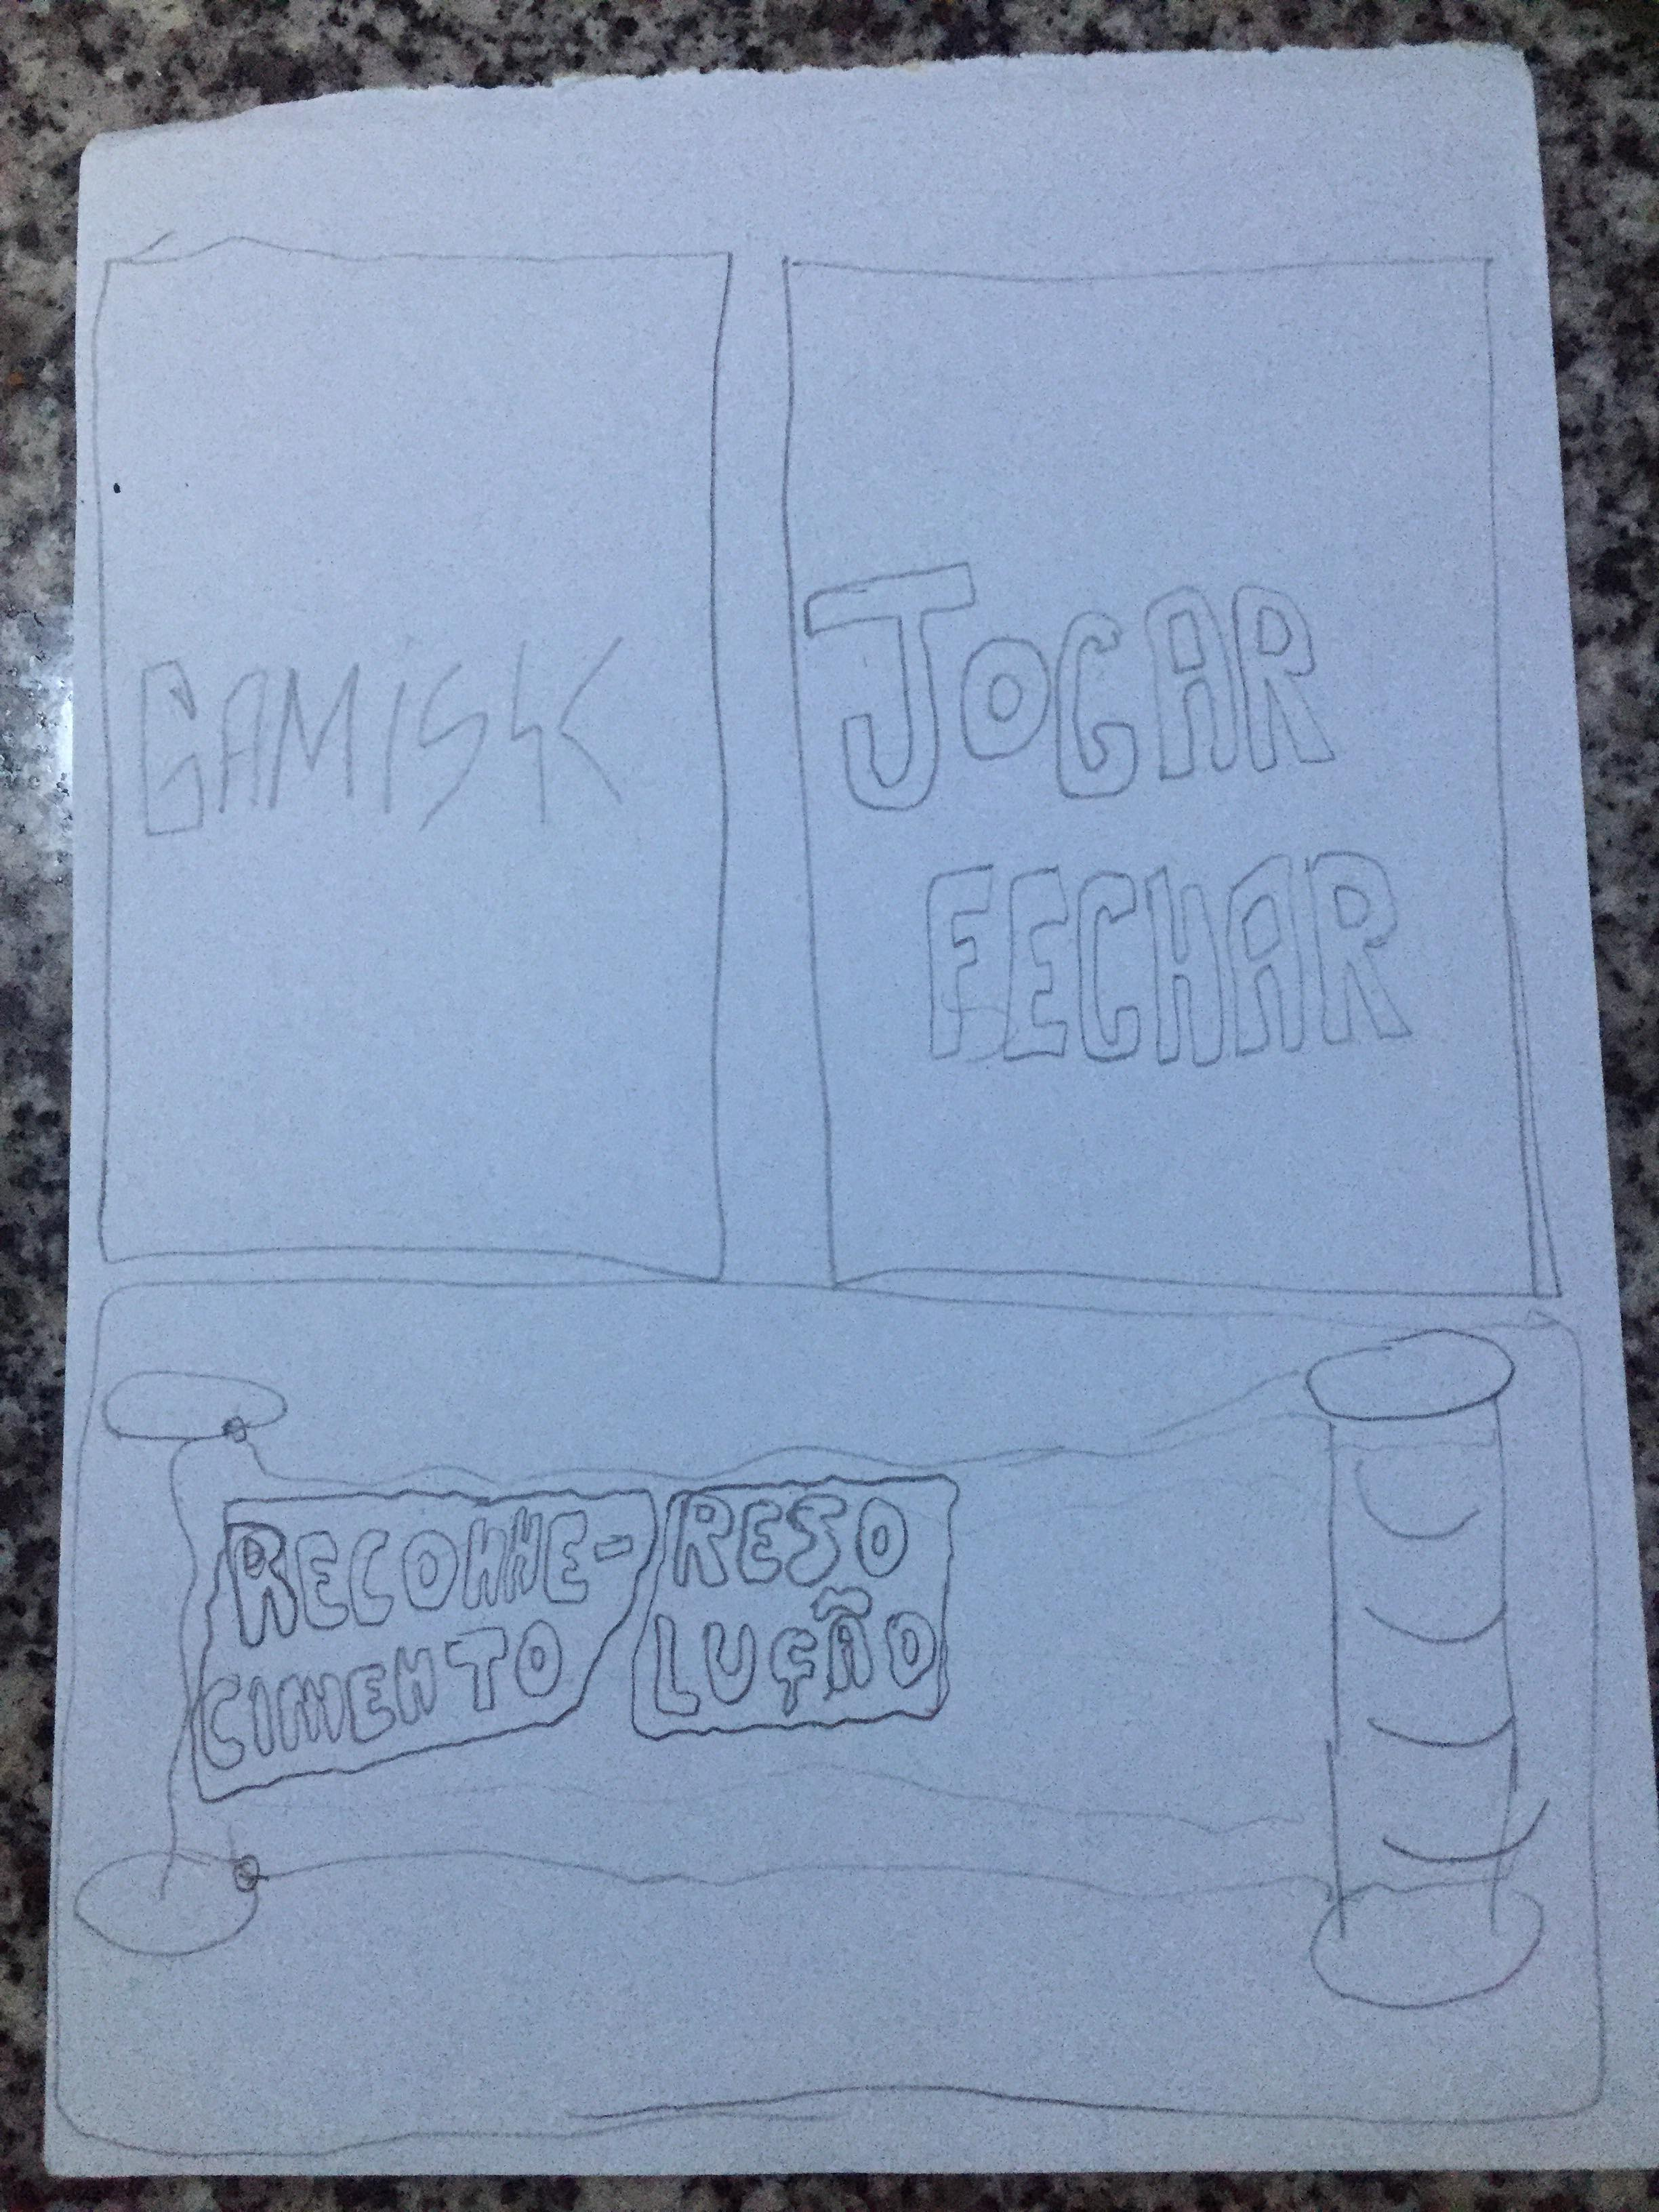
\includegraphics[scale=0.14]{figuras/prot0.jpg}
\\
\small{Fonte: do próprio autor}
\end{figure}

Na figura \ref{prot0} no primeiro retângulo em cima e à esquerda é possível ver escrito "Gamisk", que seria o primeiro nome do jogo e a primeira tela a ser apresentada ao clicar no ícone do APP. Ao lado do retângulo Gamisk à direita é possível ver escrito "Jogar" e "Fechar" que seria a segunda tela do jogo. Porém percebeu-se que não haveria necessidade das duas telas e então decidiu-se pular direto para a que apresenta "RECONHECIMENTO" E "RESOLUÇÃO". A necessidade da tela gamisk seria em caso do jogo demorar para carregar recursos, o que não acontece. A necessidade da segunda tela era para ter o botão fechar, para o jogador poder sair do jogo, porém os celulares android apresentam o botão "Home" para sair da aplicação, então viu-se desnecessário criar a funcionalidade de sair do jogo. Então ao abrir o APP o usuário já será redirecionado para escolher o módulo de jogo que deseja jogar.


A figura \ref{prot2} retrata como seria o jogo enquanto pensava-se que existiria os níveis de dificuldades fácil, médio e difícil. Depois houve o mapeamento dos níveis de dificuldade para o indicado na figura \ref{prot1}. A mudança foi então que ao invés das fases terem nome 'fácil', 'médio' e 'difícil', elas passaram a ter o nome de 'ordem', 'homogeneidade', 'tipo' e 'linearidade' e foram ordenadas de acordo com o que acreditava-se ser mais fácil para classificar até o mais difícil.


\begin{figure}[H]
\centering
\caption{Prototipação das telas dos módulos}
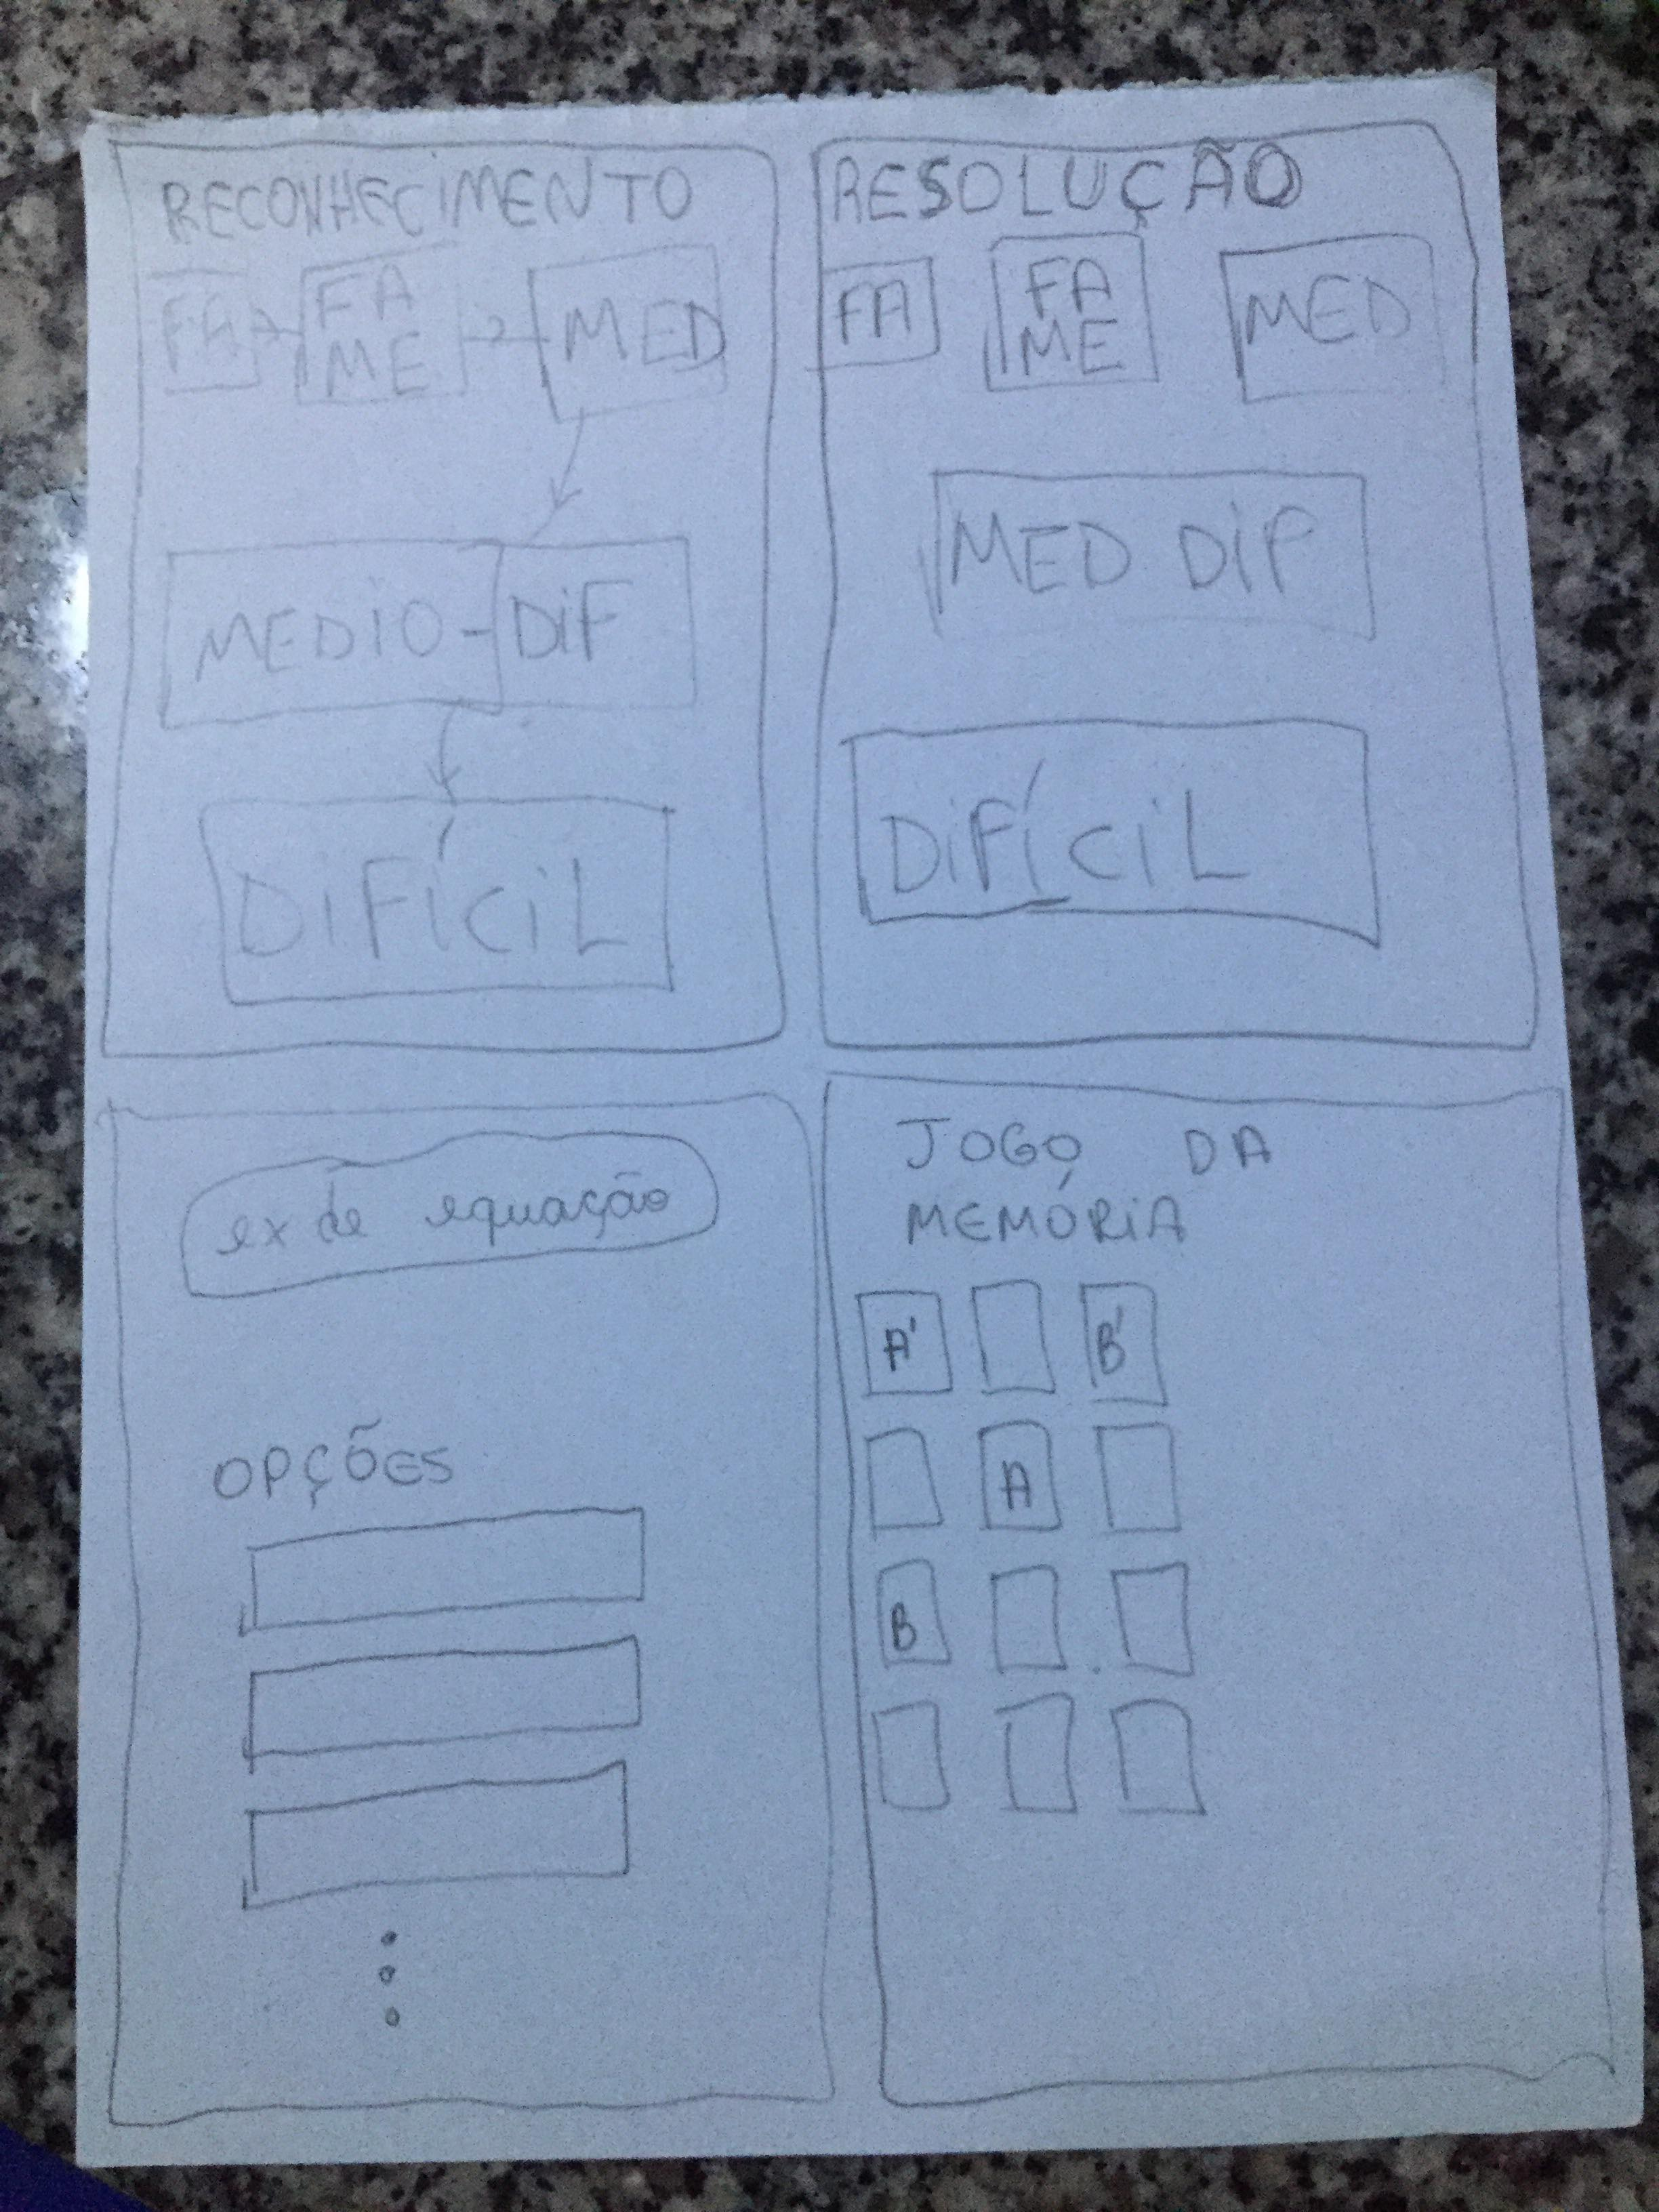
\includegraphics[scale=0.13]{figuras/prot2.jpg}
\label{prot2}
\\
\small{Fonte: do próprio autor}
\end{figure}

\begin{figure}[H]
\centering
\caption{Prototipação das telas dos módulos}
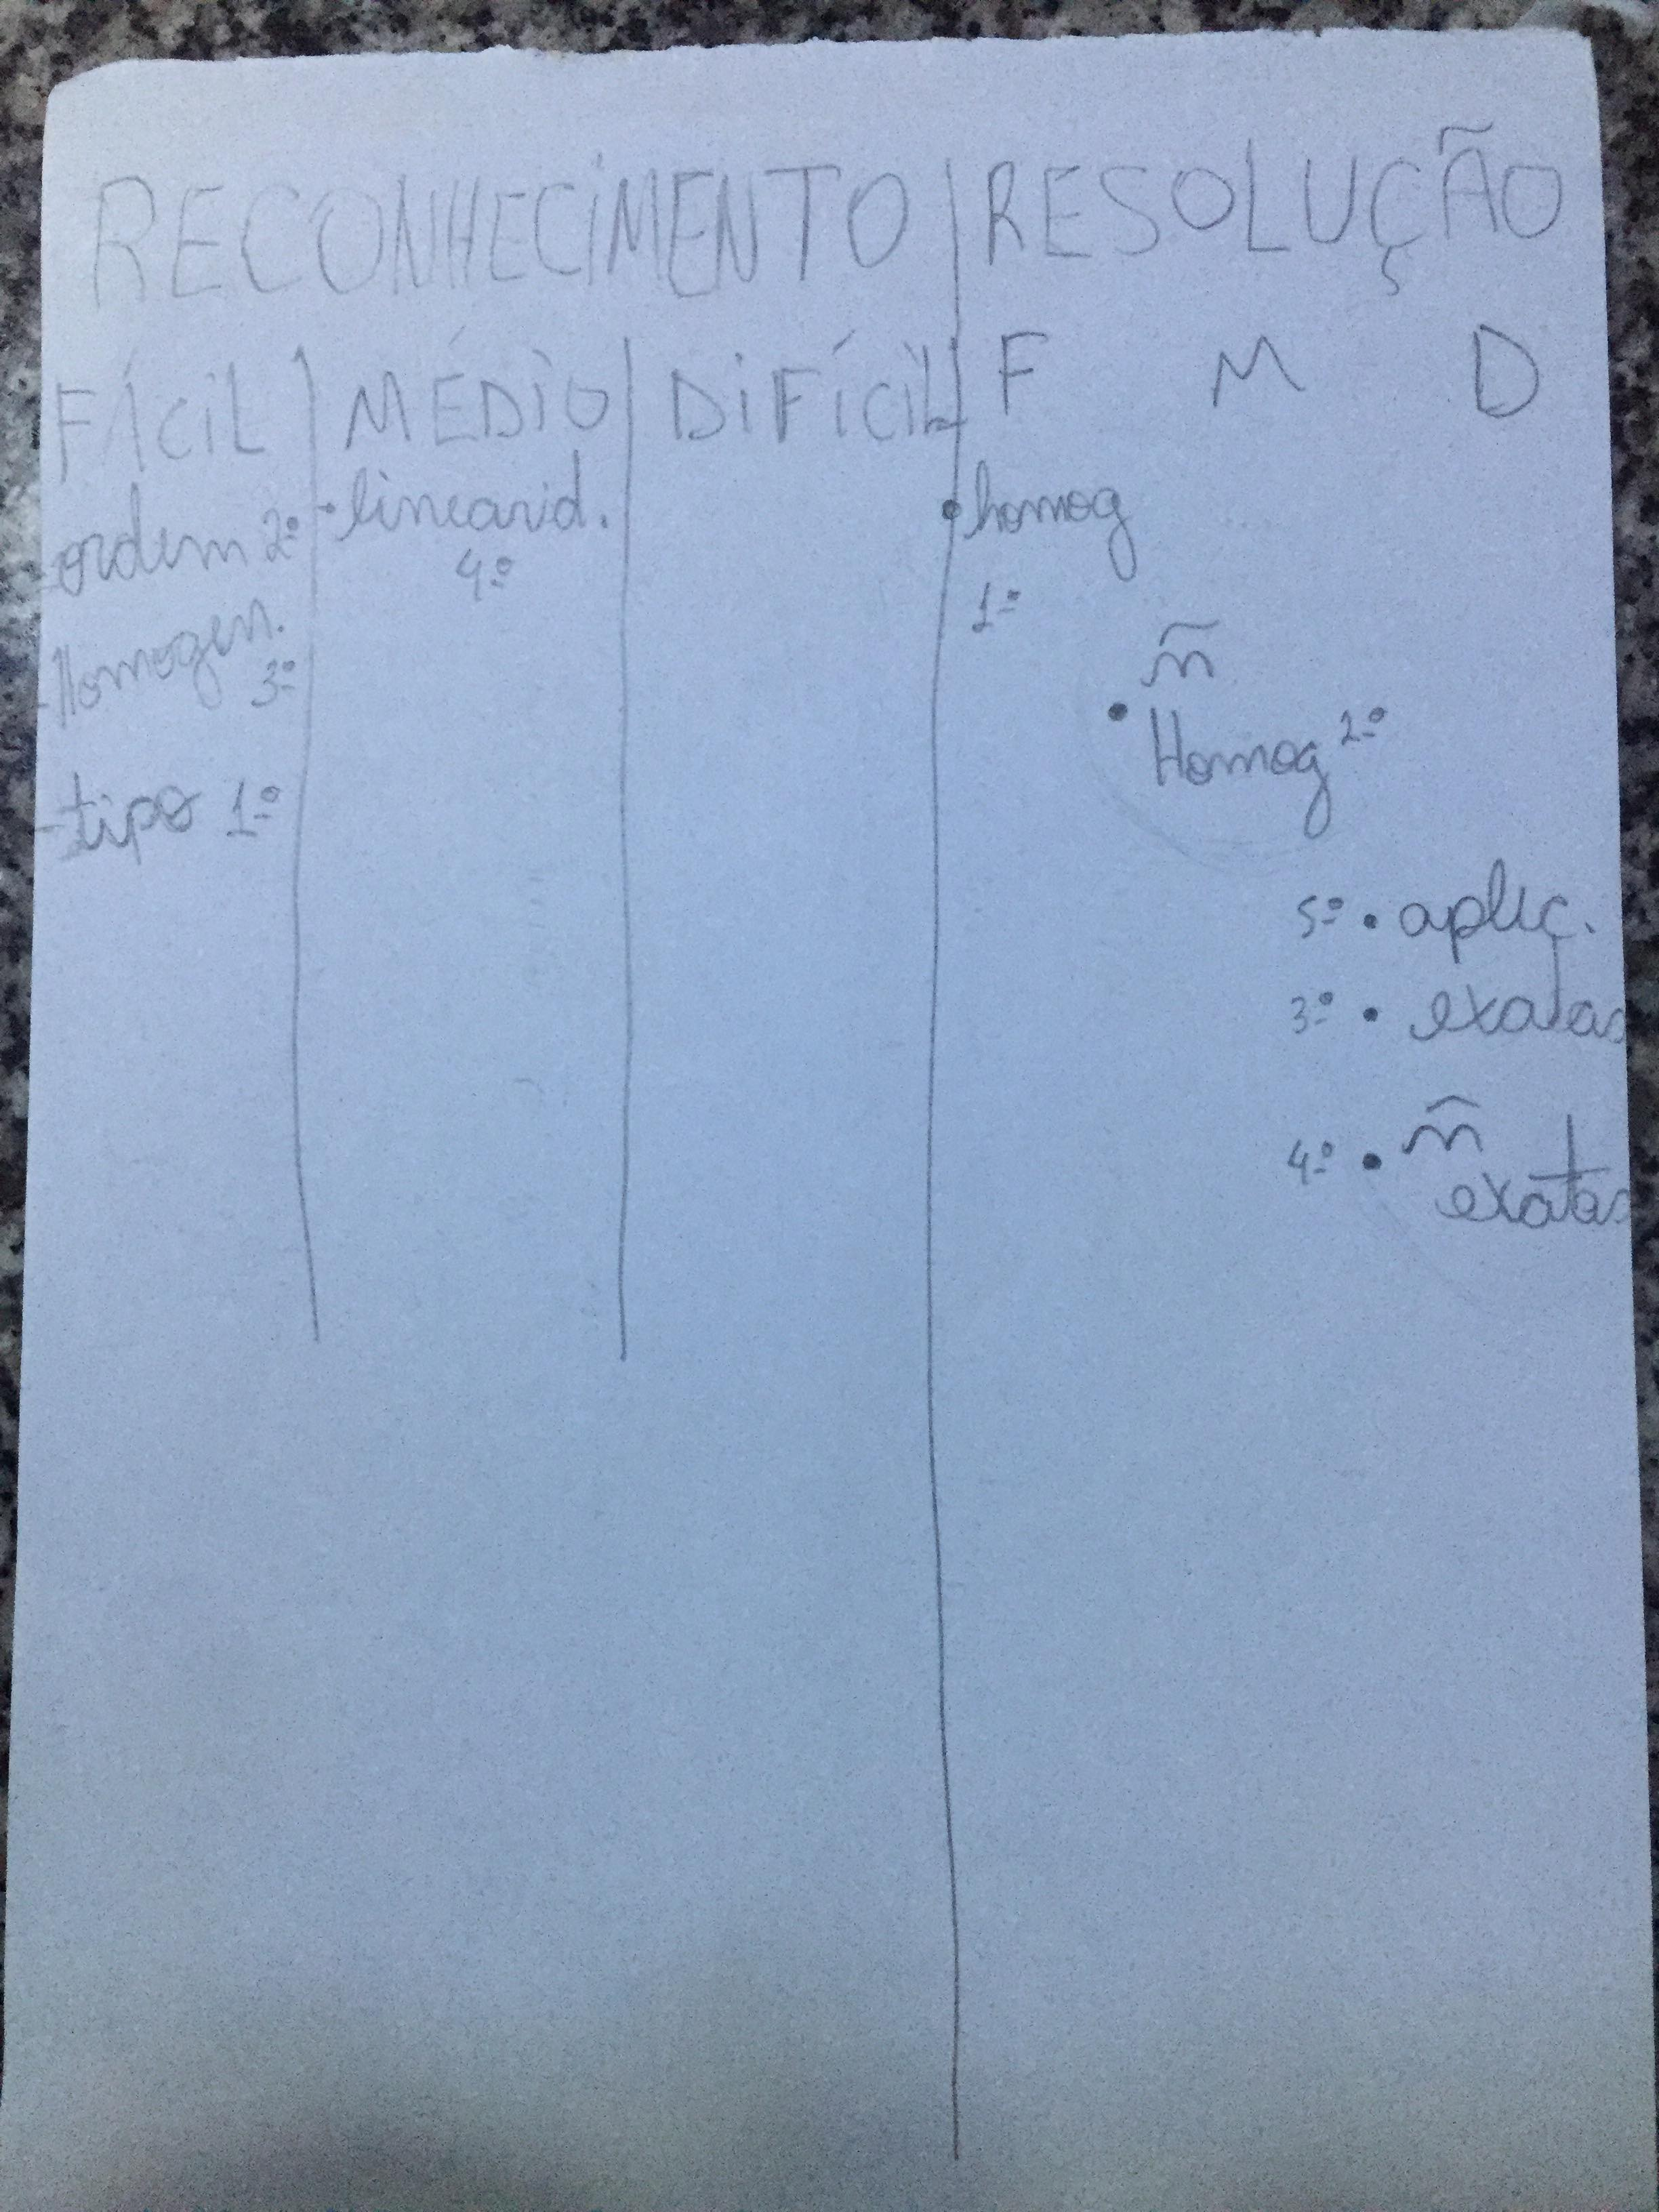
\includegraphics[scale=0.13]{figuras/prot1.jpg}
\label{prot1}
\\
\small{Fonte: do próprio autor}
\end{figure}


\section[Banco de equações]{Banco de equações}

Antes de existir o modelo definitivo dos arquivos de seeds, foi modelado a primeira versão do modelo relacional.
Este modelo tinha 5 entidades, cada uma com seus atributos. As entidades modeladas foram: 
\begin{itemize}
	\item EQUAÇÃO\_DIFERENCIAL com os atributos linearidade, separável, homogênea, exata e o id como chave primária.
	\item ORDEM com os atributos primeira, segunda, terceira, ordem superior
	\item DIFICULDADE com os atributos fácil, facilmedio, medio, mediodificil e difícil
	\item TIPO com os atributos ordinária e parcial
	\item PERGUNTA com os atributos img\_src, largura e comprimento
	\item RESPOSTA com os atributos img\_src, largura e comprimento
\end{itemize}

Houve a reflexão de criar uma entidade comum para pergunta e resposta como por exemplo IMAGEM, onde PERGUNTA e RESPOSTA herdariam as propriedades. Após outra reflexão, optou-se por não utilizar o modelo do banco porque foi julgado que o problema não era tão complexo e os dados poderiam estar guardados em pastas organizadas ao invés de um banco.

O WolfranAlpha será utilizado para fazer requisições de EDO's para serem utilizadas nas fases do jogo. Com uma chave de teste gratuita serão baixados os metadados em formato JSON através de uma API.
A API baixada do wolfran na linguagem javascript foi baixada no endereço \url{https://products.wolframalpha.com/api/libraries/javascript/}.
A chave gratuita permite 2000 requisições em um mês, com o código de série: 3GGQAT-98EG4KV6VL. Foi desenvolvido um script alimentado por um arquivo de \textit{seeds} que realiza as requisições para a API do Wolfran Alpha para ler os metadados de cada EDO's e guardar/baixar os dados necessários. Os metadados são no formato \textit{JSON}. Eles fornecem a url para a imagem .gif das equações perguntas e respostas (quando disponível), estas são utilizadas no jogo, então é necessário mapeá-las em um arquivo index.js para adicionar na pasta resource do jogo no \textit{react native} para fazer com que a internet não seja um requisito para jogar, porém para enviar dados ao servidor será necessário o acesso à internet e quando não disponível, tem como requisito avisar o jogador para tentar novamente mais tarde e espera-se então que o procedimento de zerar as estatísticas não seja acionado.

Na pasta banco existe um arquivo chamado \textbf{seeds.txt} que é o arquivo com as equações diferenciais para alimentar o banco de dados da aplicação aprEnDO. O script \textbf{equações.js} lê o arquivo de seeds equação por equação, faz a requisição para o Wolfran Alpha utilizando os códigos da pasta wolfran\_api e requisita todos os pod disponíveis (pod são os arrays de informação disponibilizados). Após ter os pods são filtradas as informações desejadas e salvas em arquivos de informações localizadas na pasta \textbf{info}. Os pods apresentam as \textit{urls} das imagens de equações de perguntas e respostas, quando existe resposta. Equações sem solução só podem ser utilizadas no primeiro módulo do jogo, o de classificação e não são incluídas no módulo de resolução. As imagens de perguntas baixadas são salvas na pasta \textbf{pergunta} e as imagens de respostas salvas na pasta \textbf{resposta}.

Com todas as informações desejadas de cada equação é possível utilizar o arquivo \textbf{estatisticas.js} que lê todos os arquivos de informação para contabilizar as informações da quantidade de equações diferenciais, quais tem resposta e quais não, quais são homogêneas, exatas, separáveis, linear, não linear, ordem1, ordem2, ordem3, ordem de 4 para cima são consideradas ordem superior, além de fazer a contagem total,também são indicados o número da equação. Essas informações são escritas num arquivo de controle para que possa ser lido pelo aplicativo aprEnDO e fazer a seleção das equações correta para renderizar, a depender do nível que a pessoa está jogando. O nome do arquivo de controle é \textbf{DADOS\_GERAIS.json}.


\section[AprEnDO]{AprEnDO}

A linguagem de programação utilizada é o nodejs com o framework react native para gerar aplicação em código nativo android. Para baixar os pacotes e fazer o controle dos mesmos está sendo utilizado o nvm e o yarn.

O ambiente de desenvolvimento usa um emulador para simular o jogo.

A pasta do jogo aprendo que encontra-se dentro da pasta desenvolvimento tem o projeto react-native com node.js e android, o package.json com as dependências, o index.js que é o ponto de entrada, os códigos fonte e os recursos. Também tem um arquivo makefile que por padrão abre o emulador de celular android, com permissão de superusuário inicia o servidor do react para desenvolvimento, cria no emulador a mais recente build do aplicativo e inicia o terminal para logs do celular emulador.

Os arquivos da pasta e uma breve explicação:
O arquivo index.js faz a importação dos módulos que são também as telas do jogo localizadas na pasta screen do código fonte em src. Também importa o módulo de navegação entra telas que precisa ser configurado para estar ciente das screens que antecedem a atual, sem a referência ao voltar a tela o jogo fecha. Uma configuração default que foi setada era para desaparecer a barra superior de navegação das telas, porém percebeu-se que em alguns celulares a barra aparecia e um pouco desconfigurada, já em outros modelos comportava como o esperado e estava invisível. 

A pasta android tem o código gerado pelo react-native o qual é um projeto padrão com os arquivos necessário para andoid, código fonte em .java, o arquivo manifest, gradle e arquivos de configuração. Algumas dependências do jogo em react native foram adicionadas manualmente no código nativo do android.

A pasta node\_modules apresenta os vários módulos do node instalados em background

A pasta resource tem as imagens de todas as equações de perguntas usada no módulo de classificação, as respostas usadas no módulo de resolução e seus arquivos index.js que mapeia o número das equações com a importação  das mesmas dentro do jogo, a importação só se da porquê todas as imagens já possuem o termo “require(‘numero da equação’)” que é pré-processada antes da escolha da equação aleatória a ser importada dentro da fase. Outro arquivo importante que tem nessa pasta é o \textbf{DADOS\_GERAIS.json} que possui os metadados das equações, quanto à todas classificações, tipo, ordem, homogeneidade e etc.

Foram desenhados processos para entender o fluxo do jogo. O primeiro processo é uma visão geral.

\begin{figure}[H]
\centering
\caption{Processo geral do jogo aprEnDO}
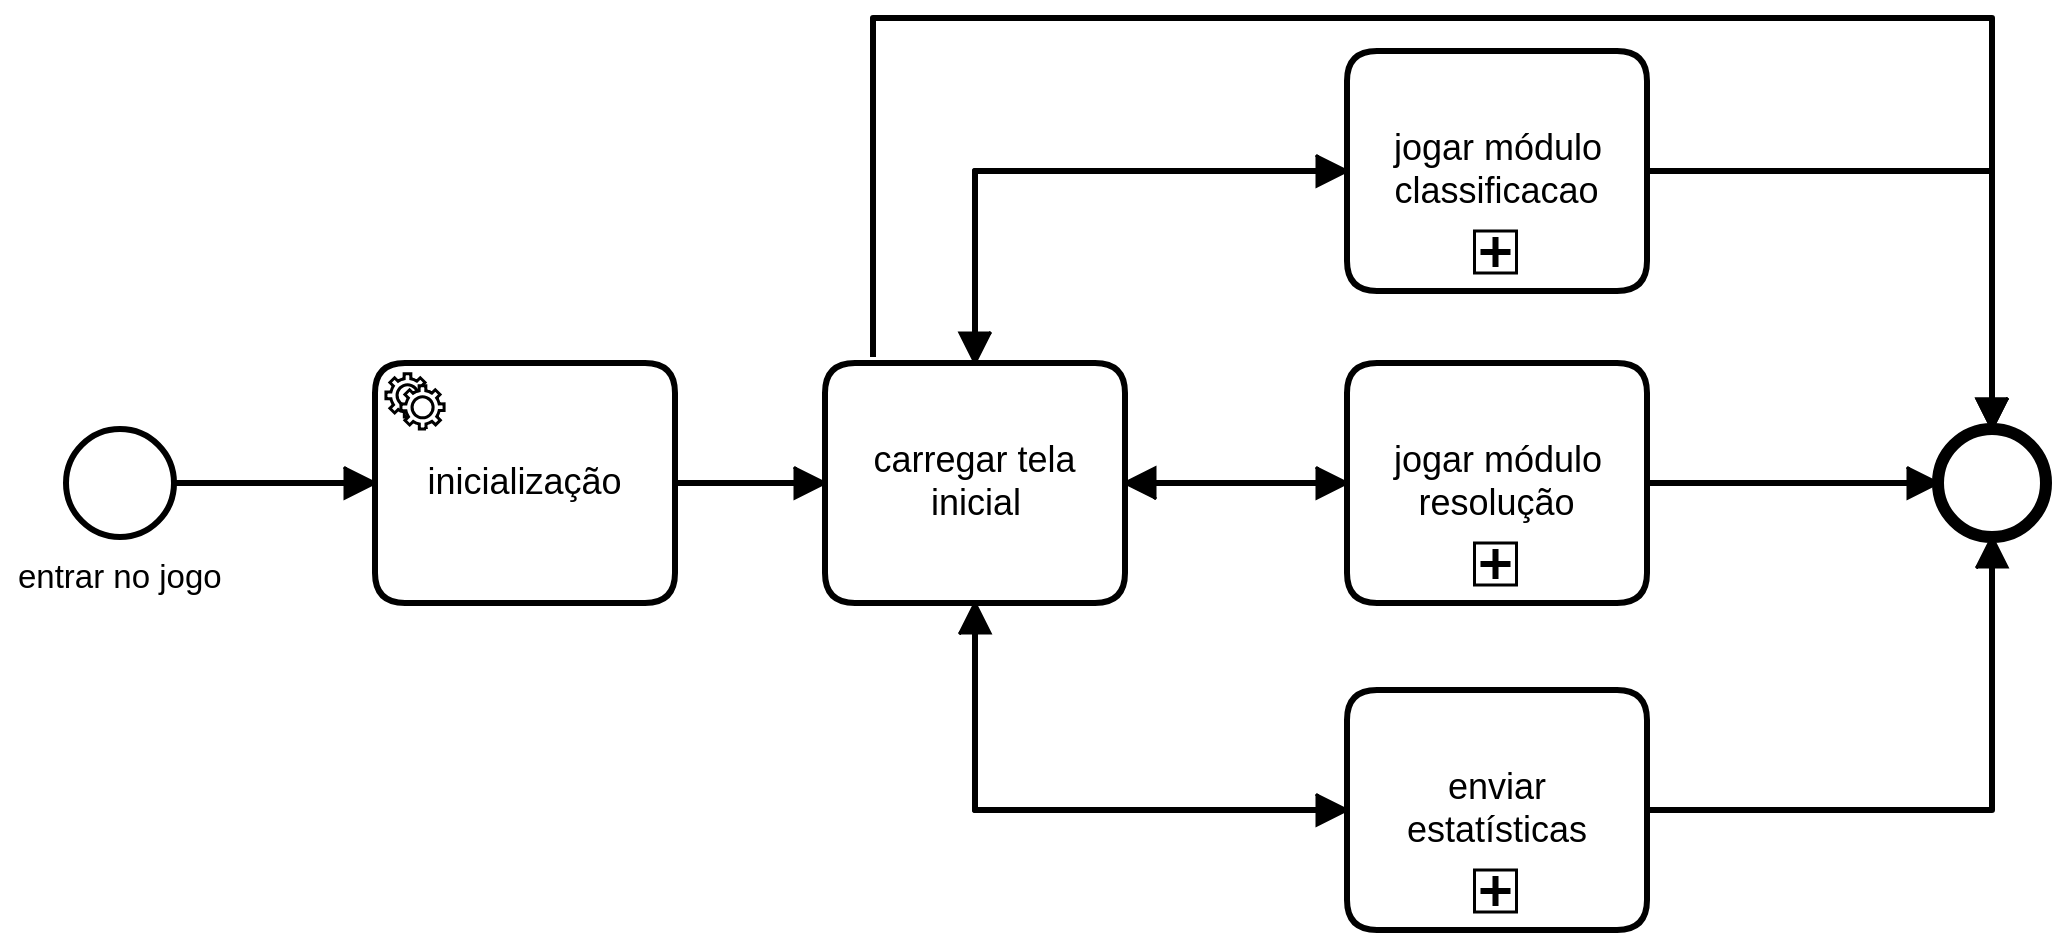
\includegraphics[scale=0.2]{figuras/processos/processo_geral.png}
\label{pg}
\\
\small{Fonte: do próprio autor}
\end{figure}

Na figura \ref{pg} mostra-se que ao entrar no APP a primeira atividade é um script do sistema, assim que este termina é carregada a tela inicial que permite ao usuário jogar o módulo de classificação, jogar o módulo de resolução, enviar estatatísticas ou simplesmente sair do jogo sem fazer nada.

A primeira macro-atividade é a inicialização, indicada na figura \ref{inic}.

\begin{figure}[H]
\centering
\caption{Processo de inicialização do jogo aprEnDO}
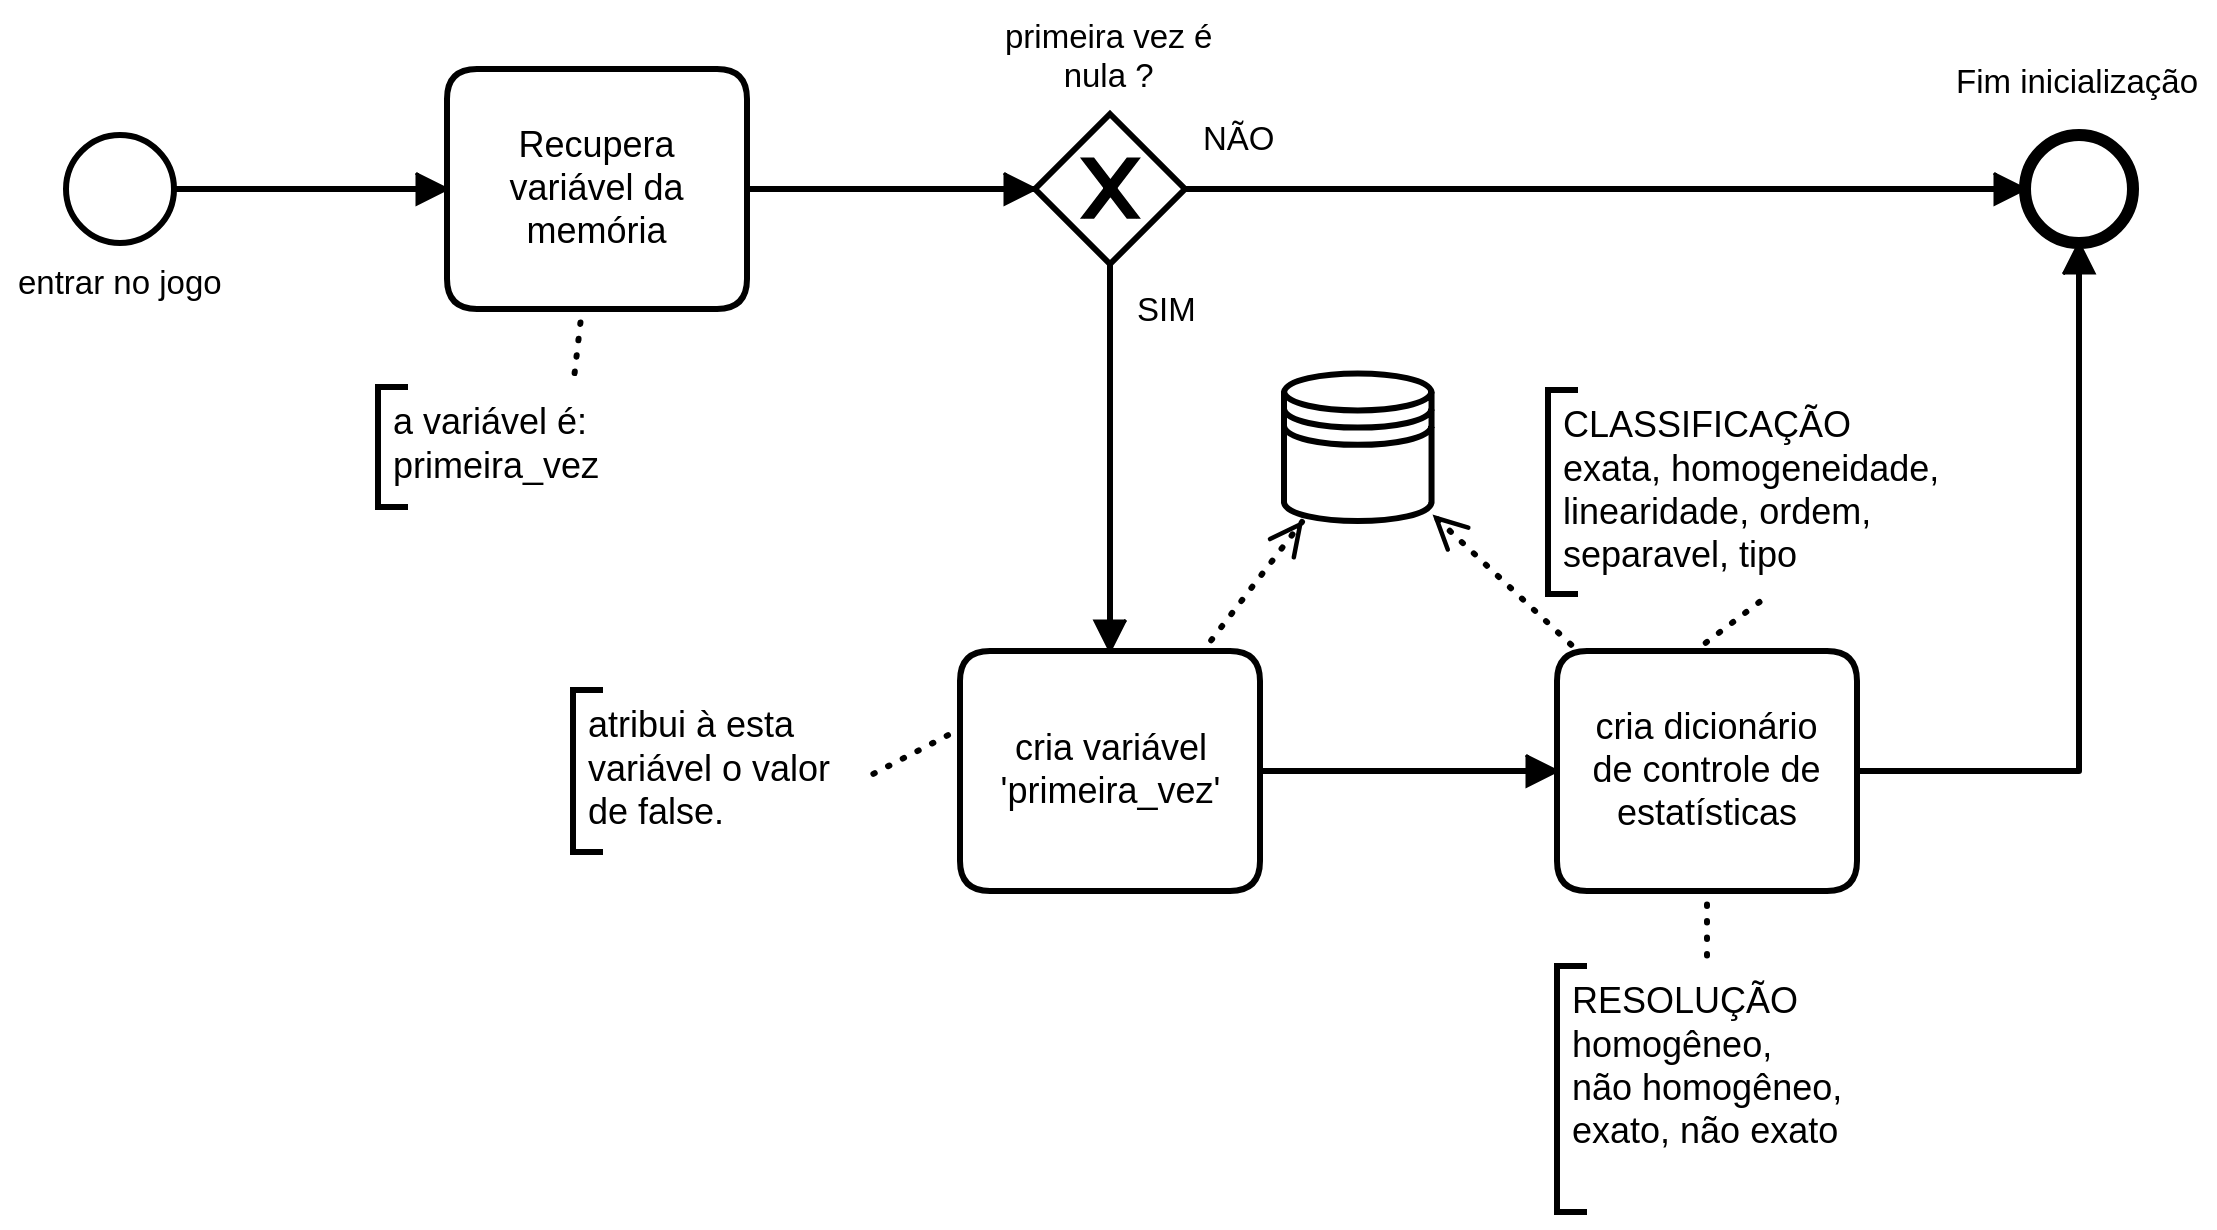
\includegraphics[scale=0.2]{figuras/processos/proccesso_inicializacao.png}
\label{inic}
\small{Fonte: do próprio autor}
\end{figure}

O processo \ref{inic} recupera a variável 'primeira\_vez' da memória, caso a variável exista e tenha o valor de 'falso' significa que o usuário já jogou outras vezes, então o processo termina. Caso seja realmente a primeira vez do usúário é necessário criar a variável 'primeira\_vez' para sinalizar que não é mais a primeira vez. Também é criado a estrutura de estatísticas para classificação e resolução e persistida no banco de dados do celular.

A segunda macro\-atividade é o processo de jogar o módulo de classificação, nele o usuário precisa escolher alguma fase de classificação. A figura \ref{class_proc} mostra quais são as possíveis ações a serem tomadas pelo jogador.

\begin{figure}[H]
\centering
\caption{Processo de jogo de classificação}
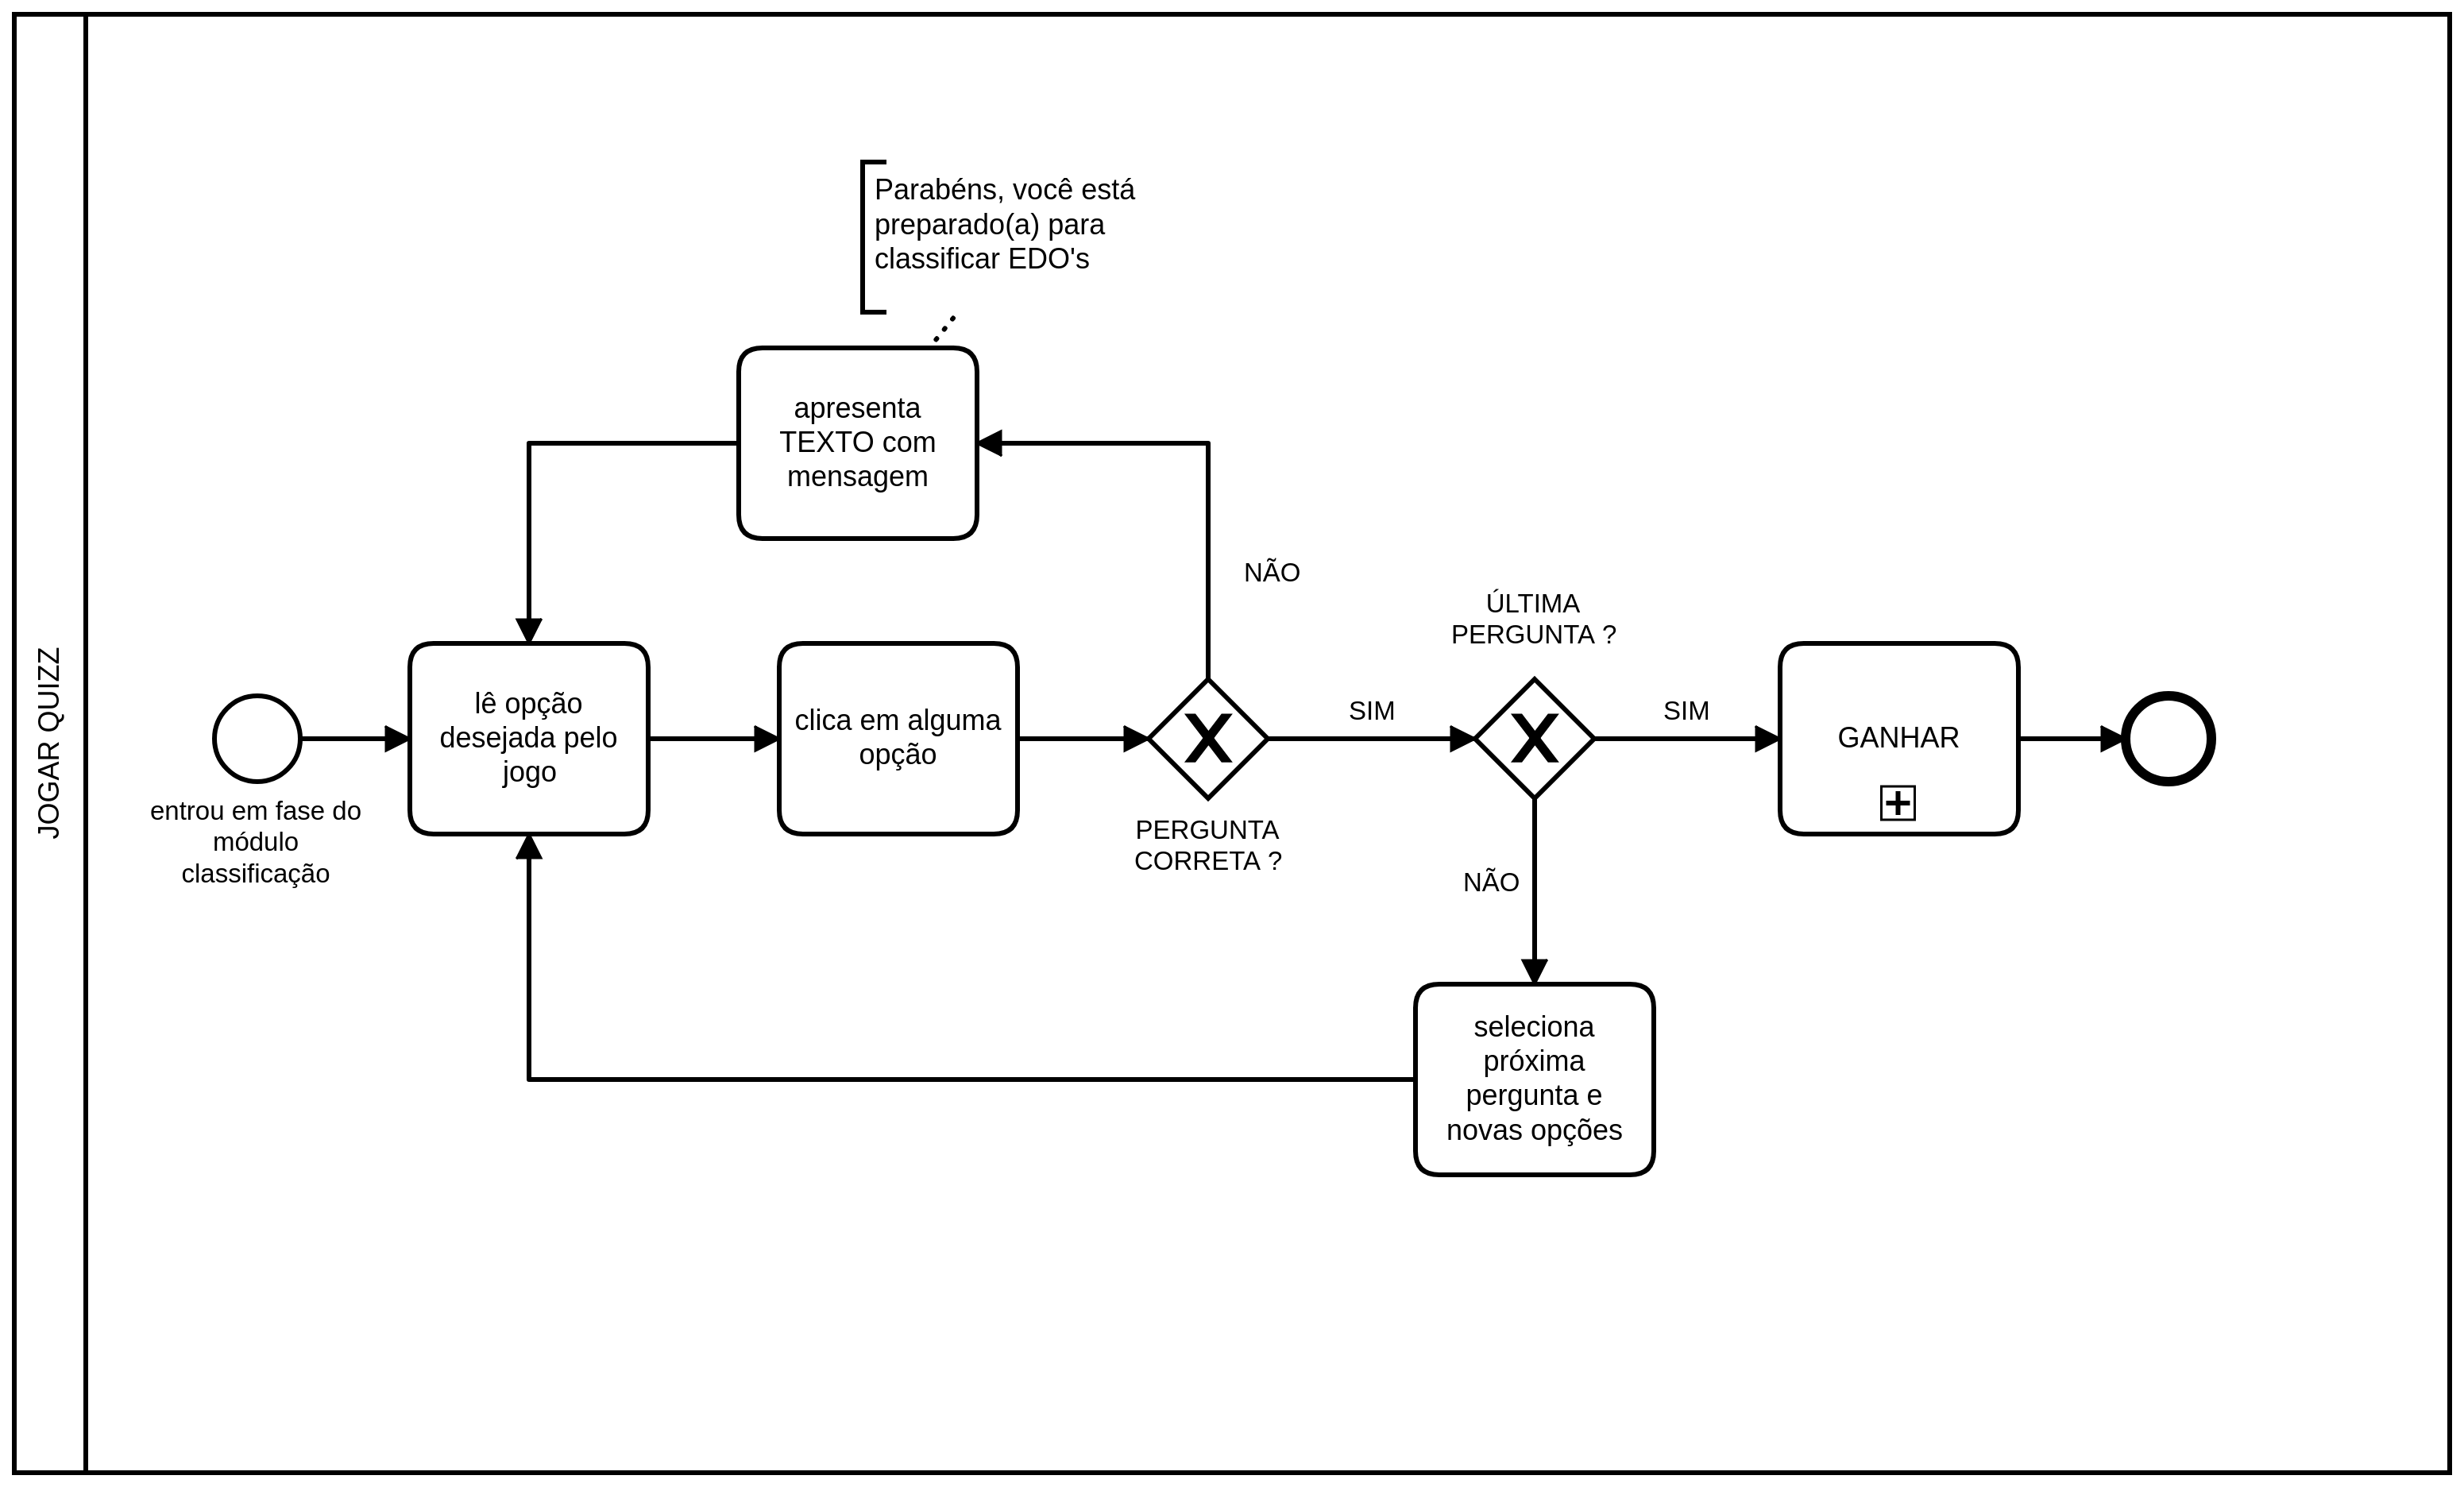
\includegraphics[scale=0.15]{figuras/processos/processo_classificacao.png}
\label{class_proc}
\small{Fonte: do próprio autor}
\end{figure}

Ámbos os módulos \ref{class_proc} e \ref{res_proc} podem ativar o processo da figura \ref{ganhar_proc} que consiste em armazenar as estatísticas de mais uma vitória nos dados do celular para que possam ser enviados ao servidor de coleta.


\begin{figure}[H]
\centering
\caption{Processo de ganhar uma fase}
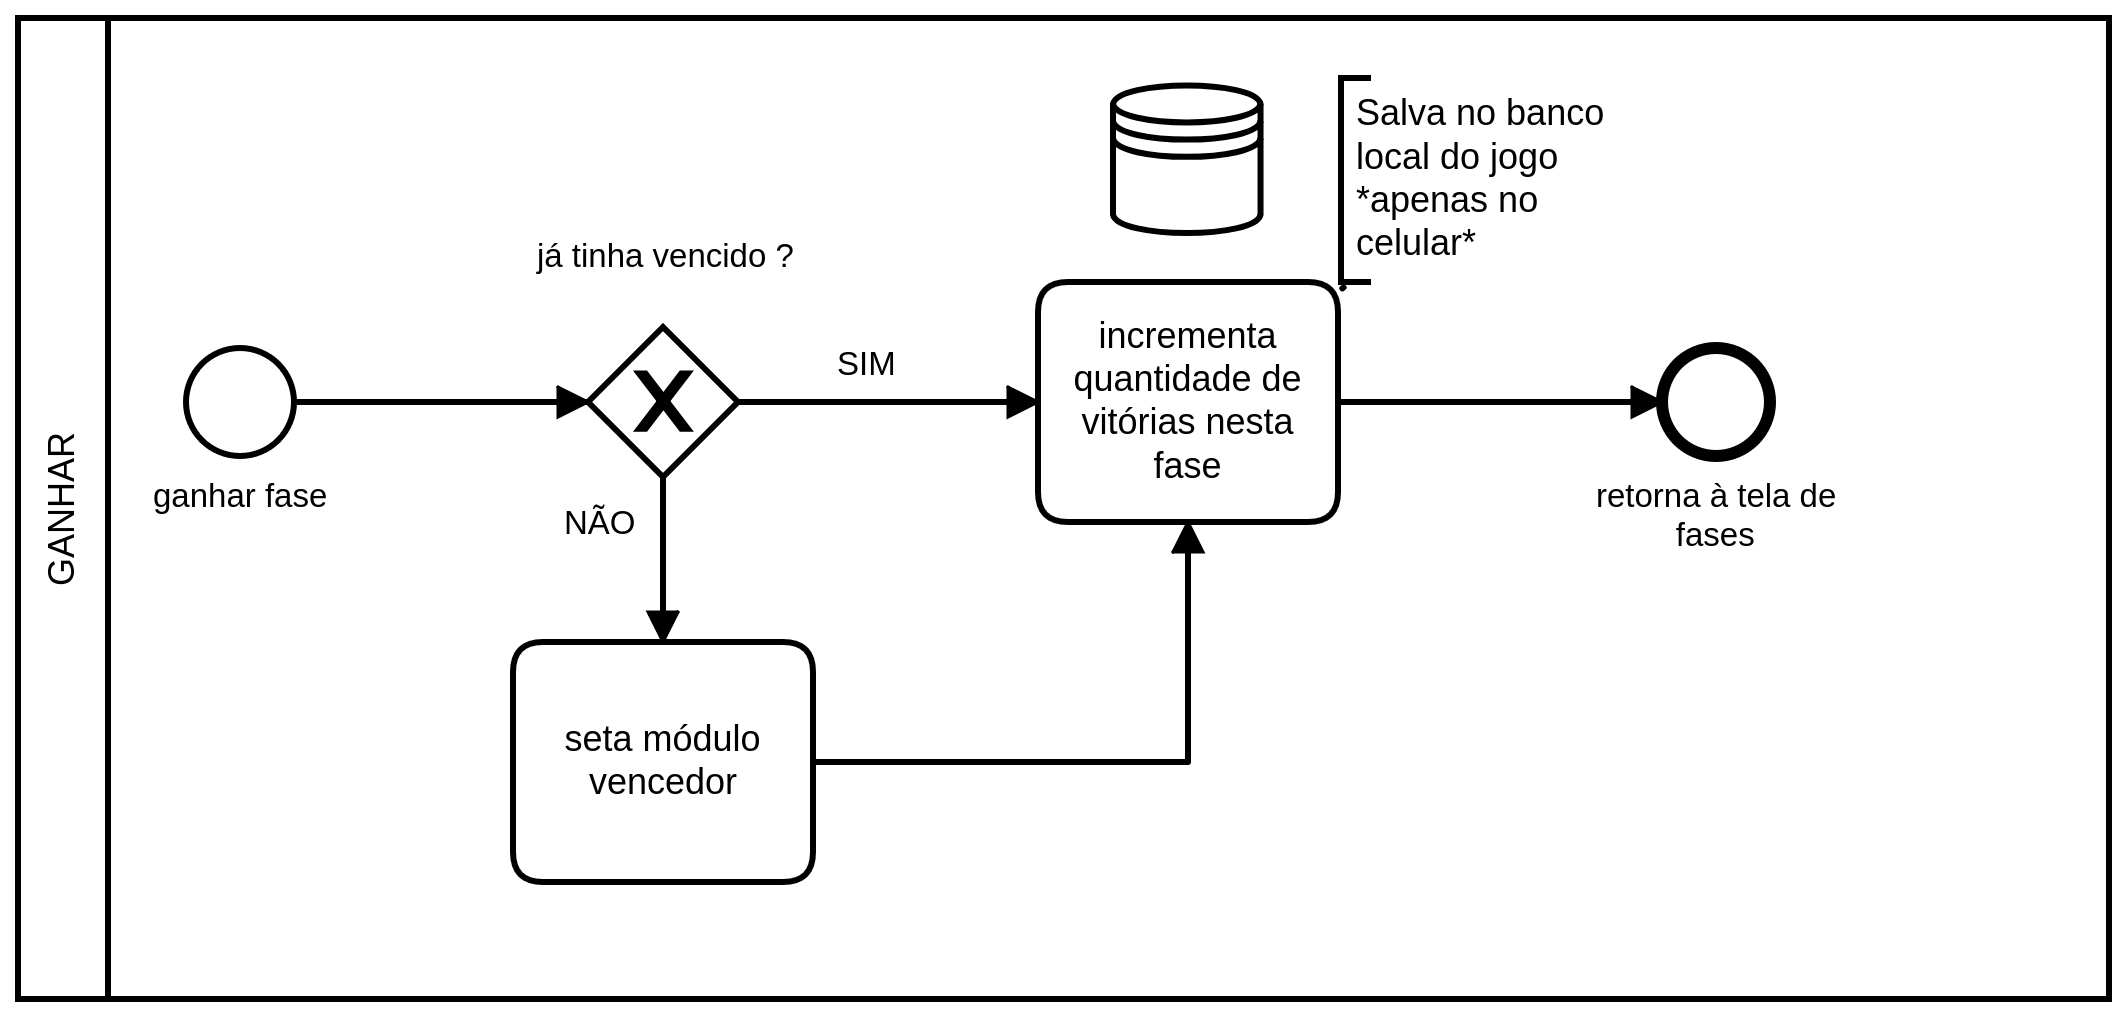
\includegraphics[scale=0.23]{figuras/processos/processo_ganhar.png}
\label{ganhar_proc}
\small{Fonte: do próprio autor}
\end{figure}


\begin{figure}[H]
\centering
\caption{Processo de jogo de resolução}
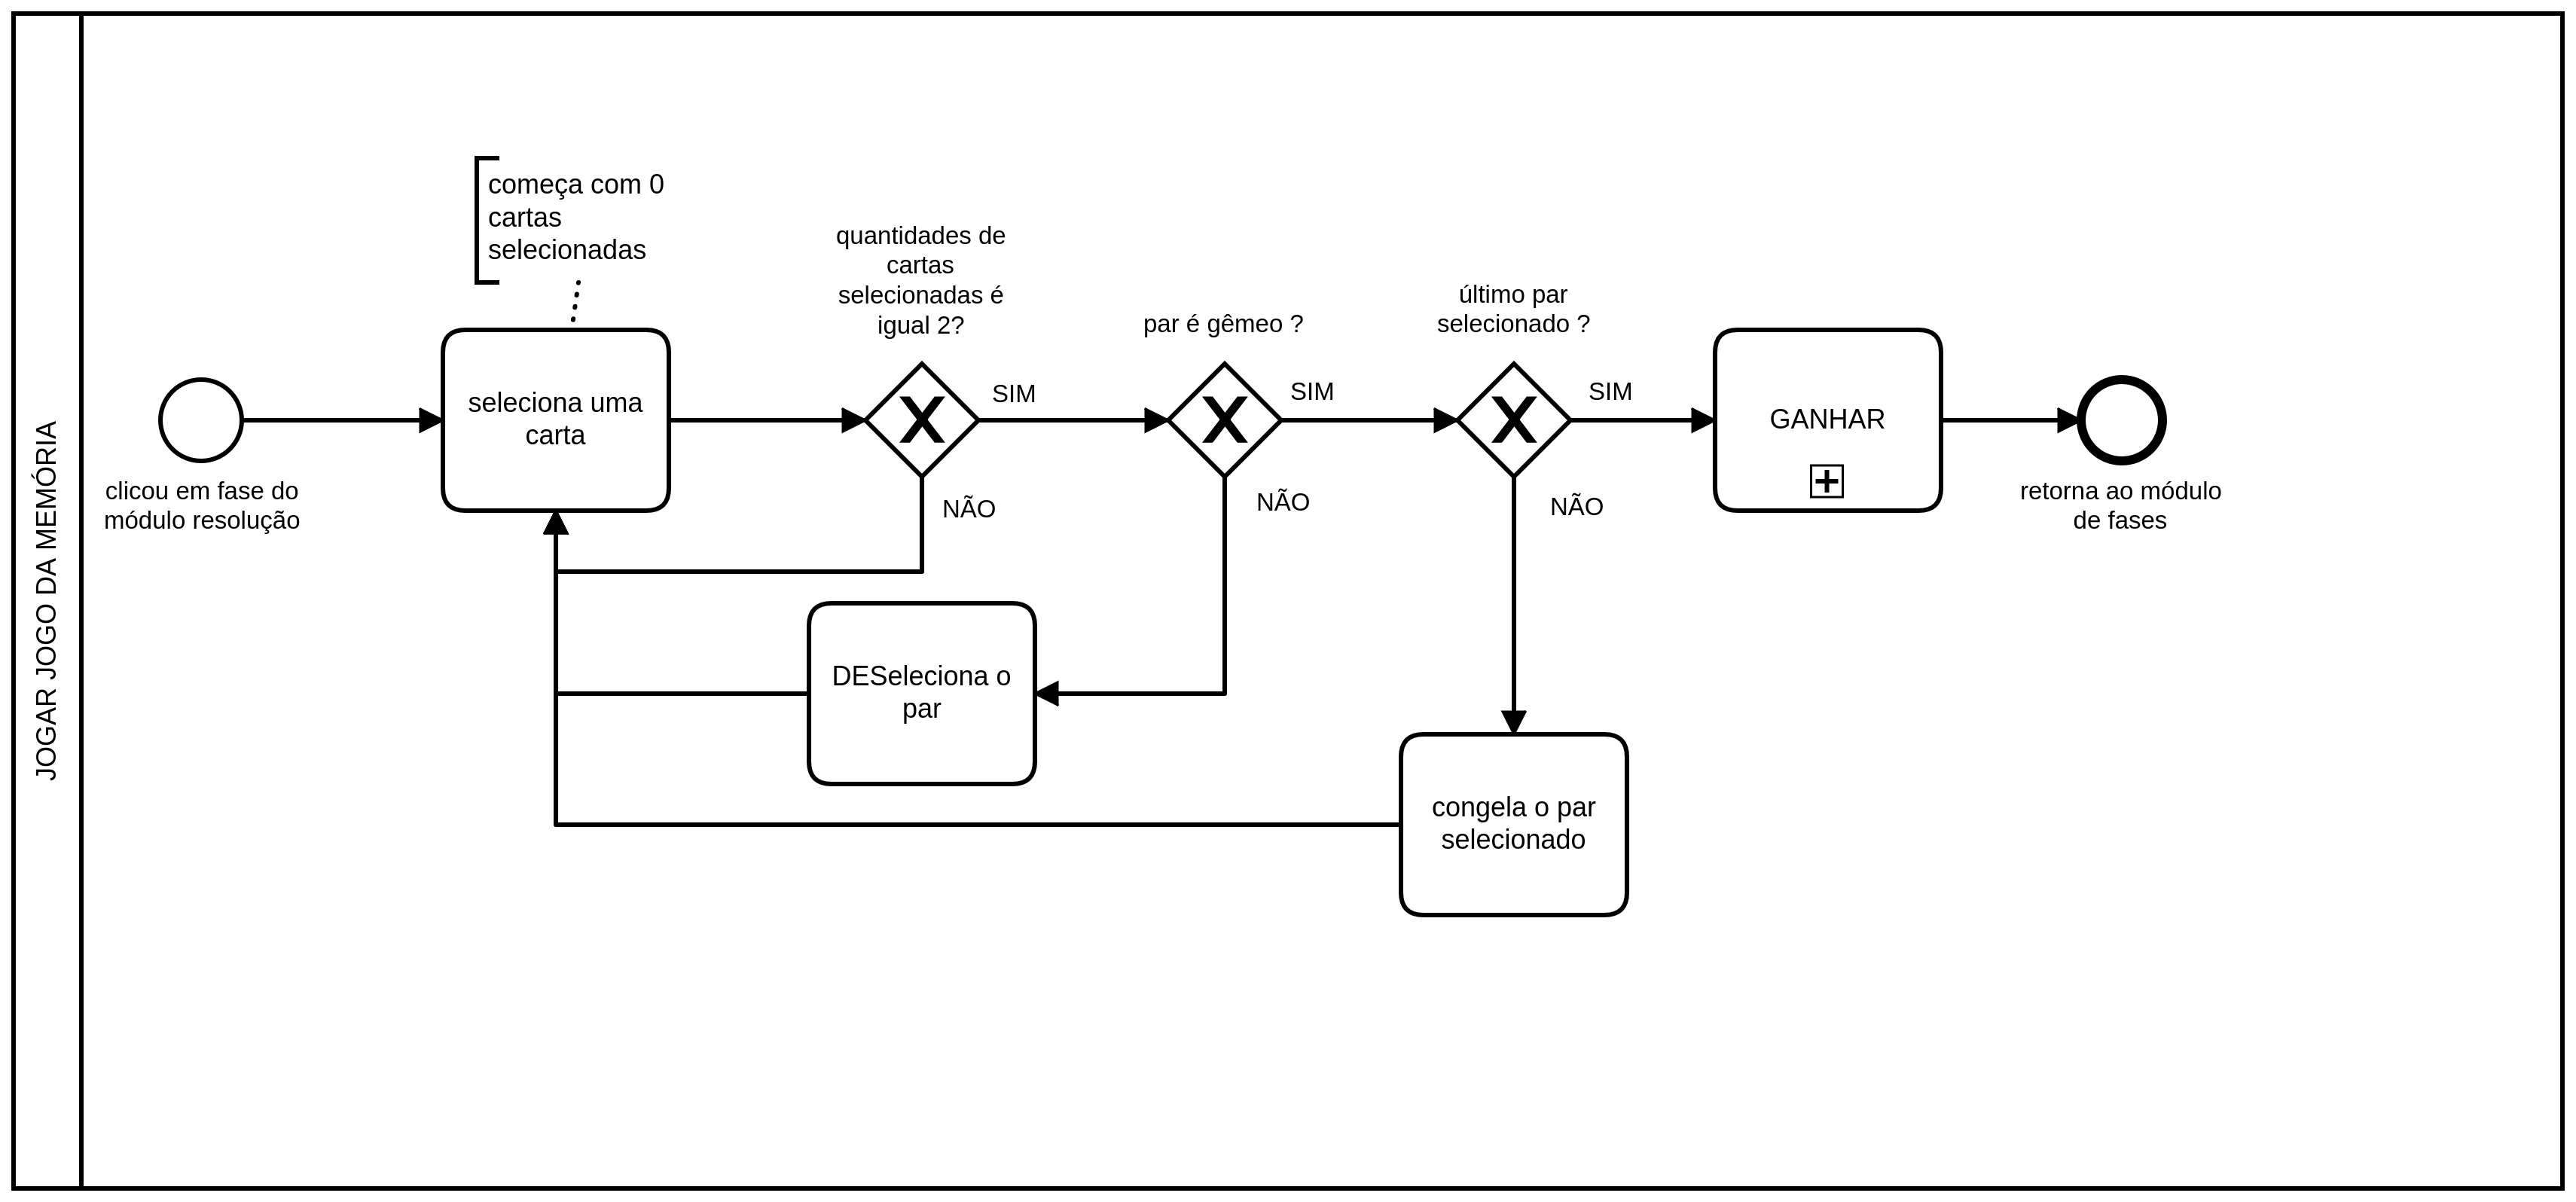
\includegraphics[scale=0.15]{figuras/processos/processo_resolucao.png}
\label{res_proc}
\small{Fonte: do próprio autor}
\end{figure}

A quarta macro-atividade envolve o envio de estatísticas de jogo para um servidor de análise e coleta. O processo é detalhado na figura \ref{envio_estatisticas}.

\begin{figure}[H]
\centering
\caption{Envio de estatísticas}
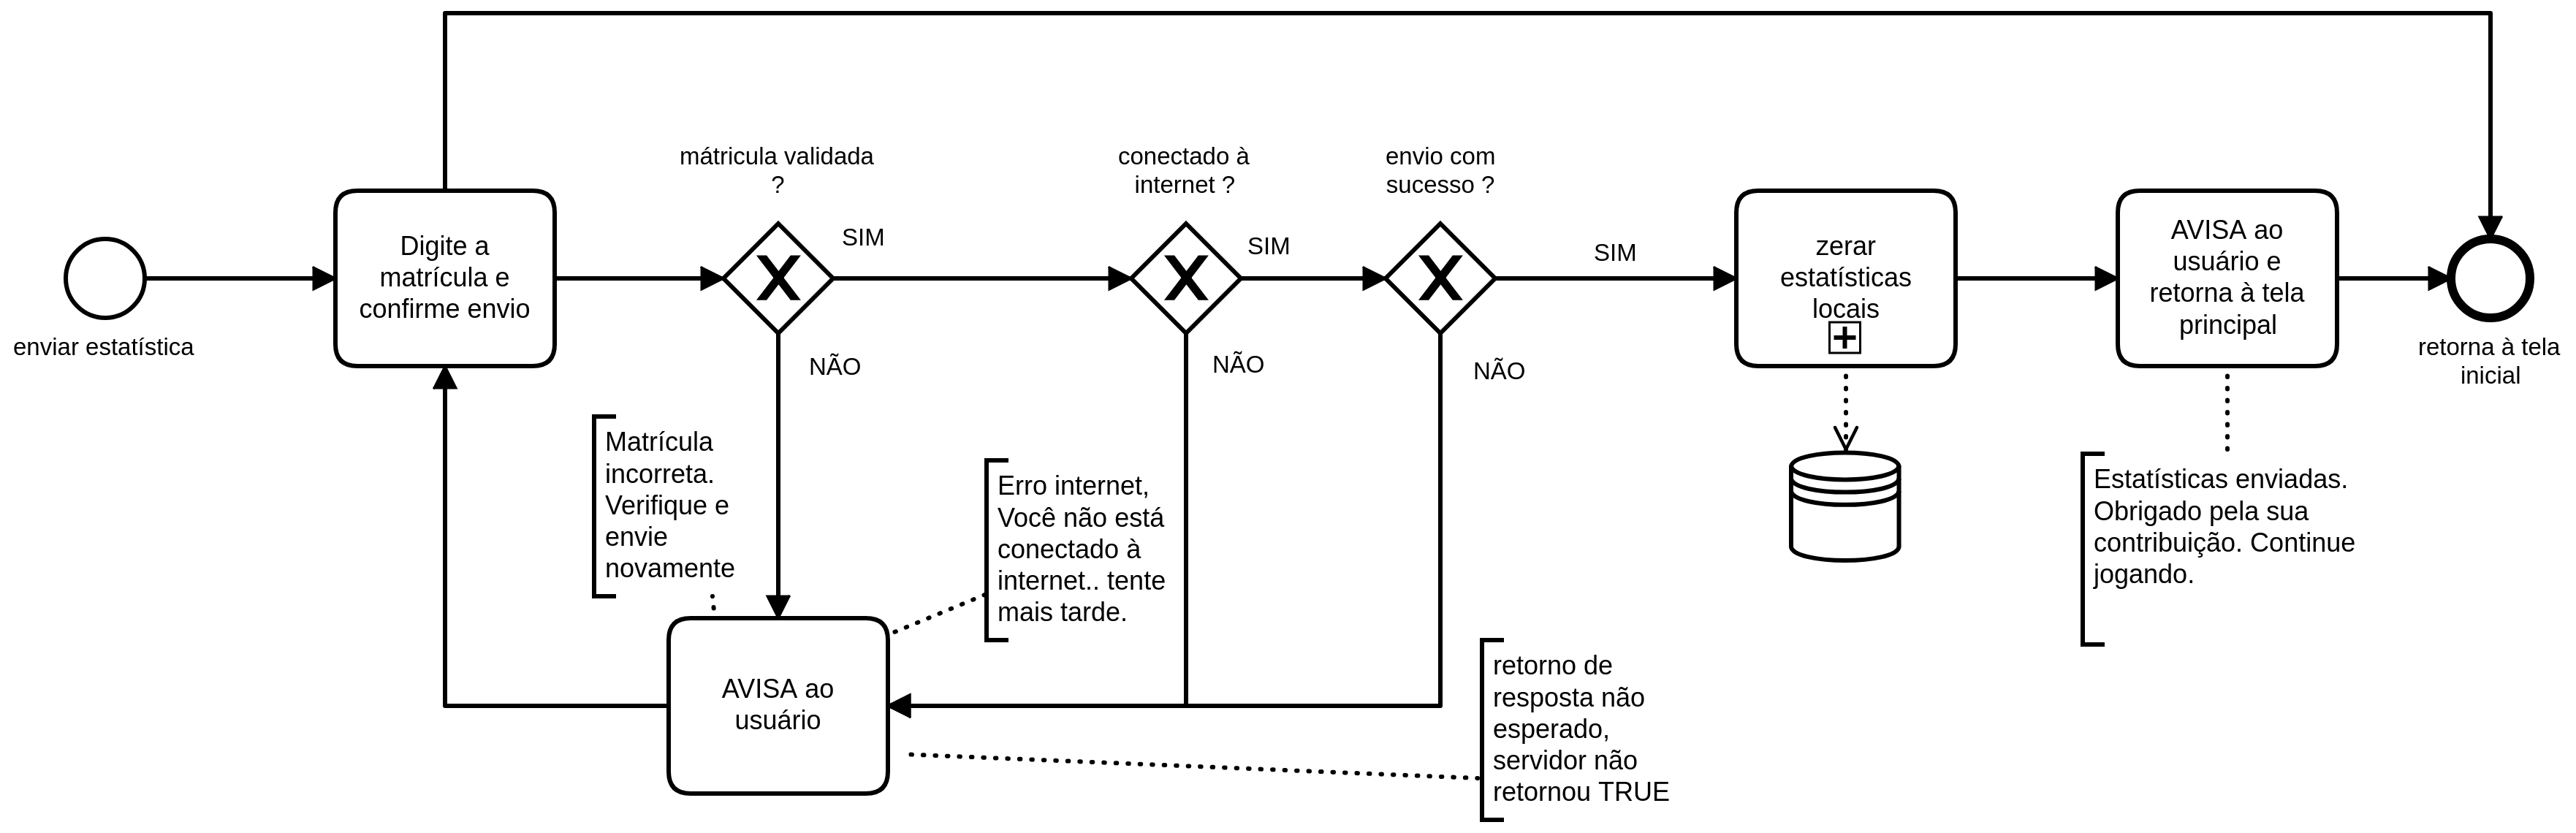
\includegraphics[width=\textwidth,height=\textheight,keepaspectratio]{figuras/processos/processo_enviar_estatisticas.png}
\label{envio_estatisticas}
\small{Fonte: do próprio autor}
\end{figure}

É necessário que o jogador digite sua matrícula corretamenta, pois esta será validada com a quantidade de 8 algarismos. Caso a matrícula seja validada e haja a conexão com a internet ocorrerá o envio dos dados, qualquer erro pelo caminho haverá o aviso específico ao jogador. Após a persistência dos dados no servidor, os dados locais são zerados para que não sejam redundantes no próximo envio. O processo de zerar estatísticas é apresentado na figura \ref{zerar_estatisticas}. 

\begin{figure}[H]
\centering
\caption{Zerar estatísticas após envio}
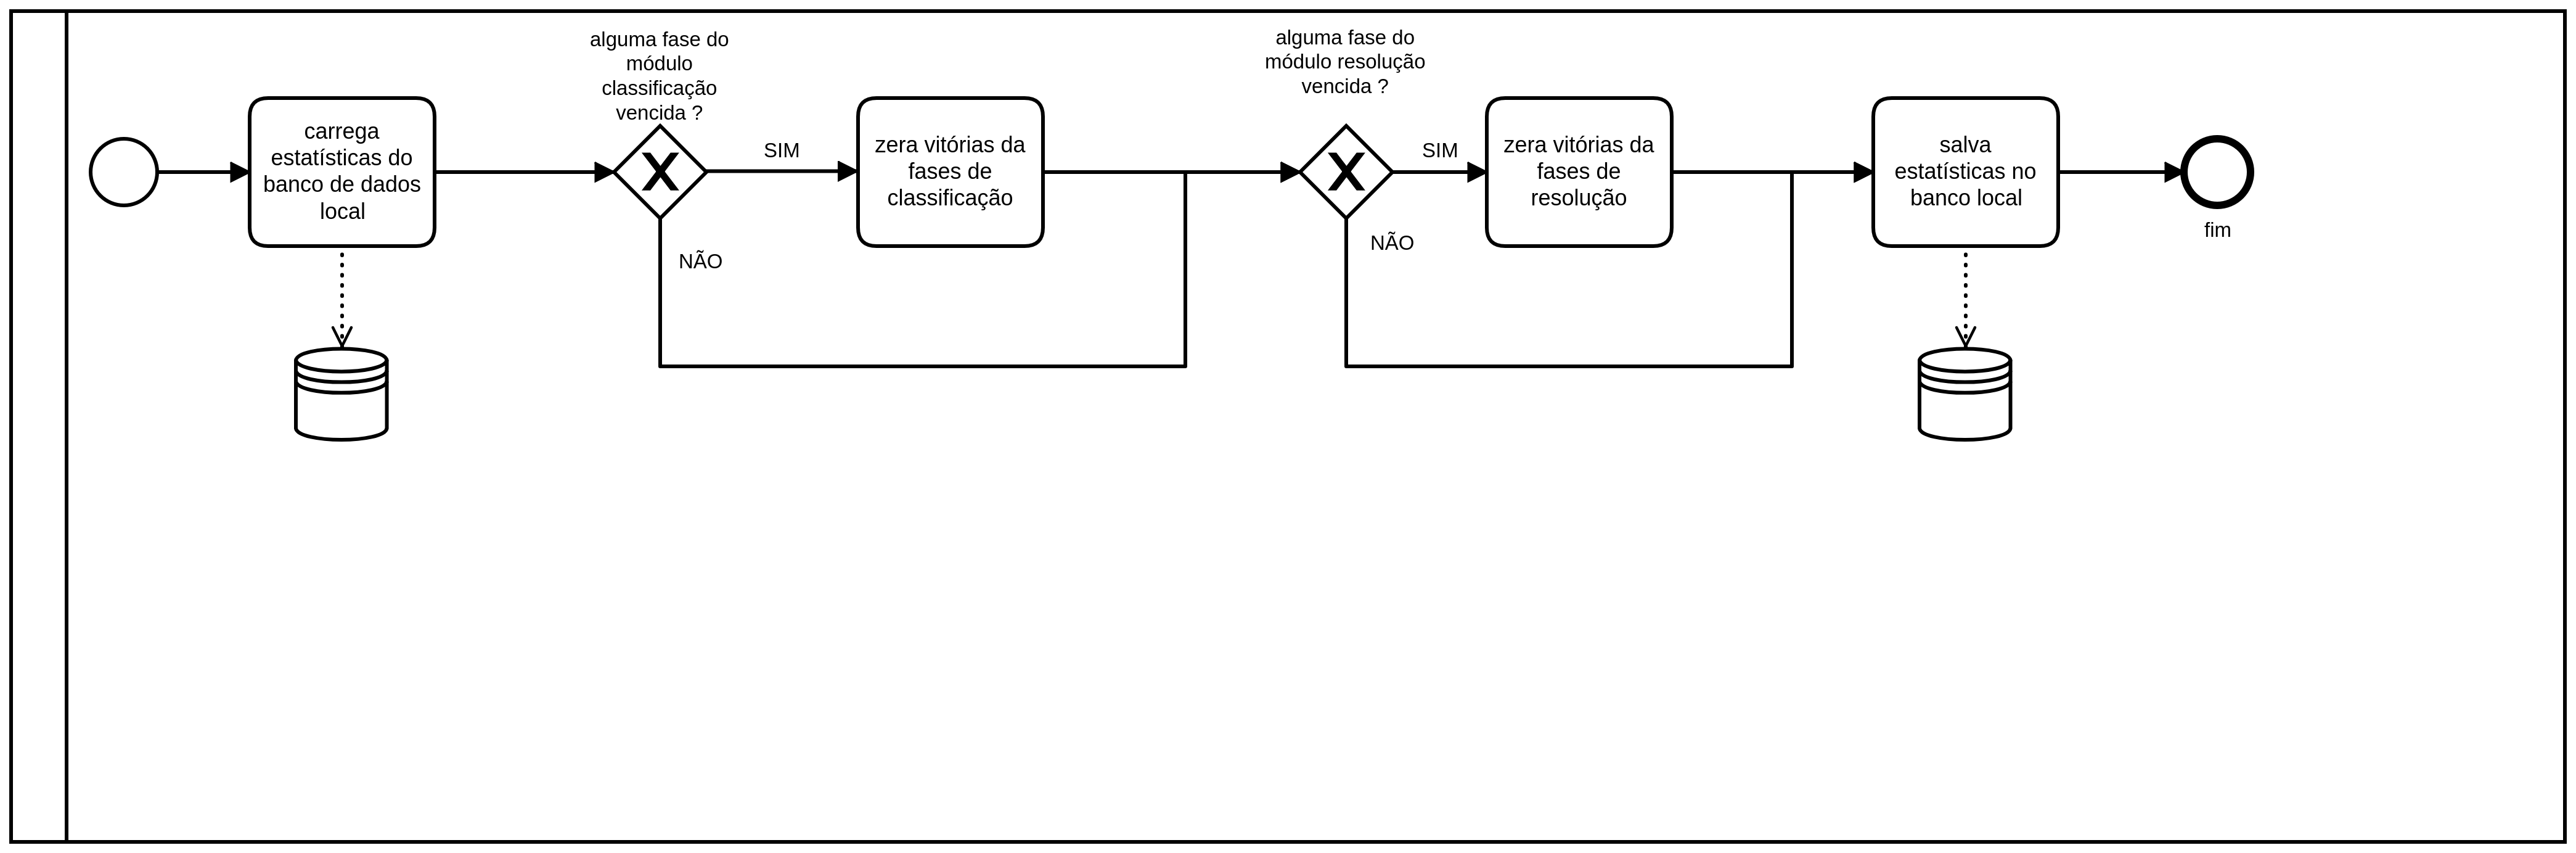
\includegraphics[width=\textwidth,height=\textheight,keepaspectratio]{figuras/processos/processo_zerar_estatisticas.png}
\label{zerar_estatisticas}
\small{Fonte: do próprio autor}
\end{figure}

Zerar estatísticas percorre as fases de classificação e resolução verificando qual fase já foi vencidade ao menos uma vez e trocando o valor atual para 0. Após o loop nos módulos os dados são persistidos na memória do celular.

Outro artefato de documentação desenvolvido foi o diagrama de classes. Este foi modelado de modo a facilitar o desenvolvimento e o entendimento da pasta src, pois deu uma guiada no que precisava ser feito e como as classes do jogo e os componentes se relacionam. 

\begin{figure}[H]
\centering
\caption{Diagrama de Classe do AprEnDO}
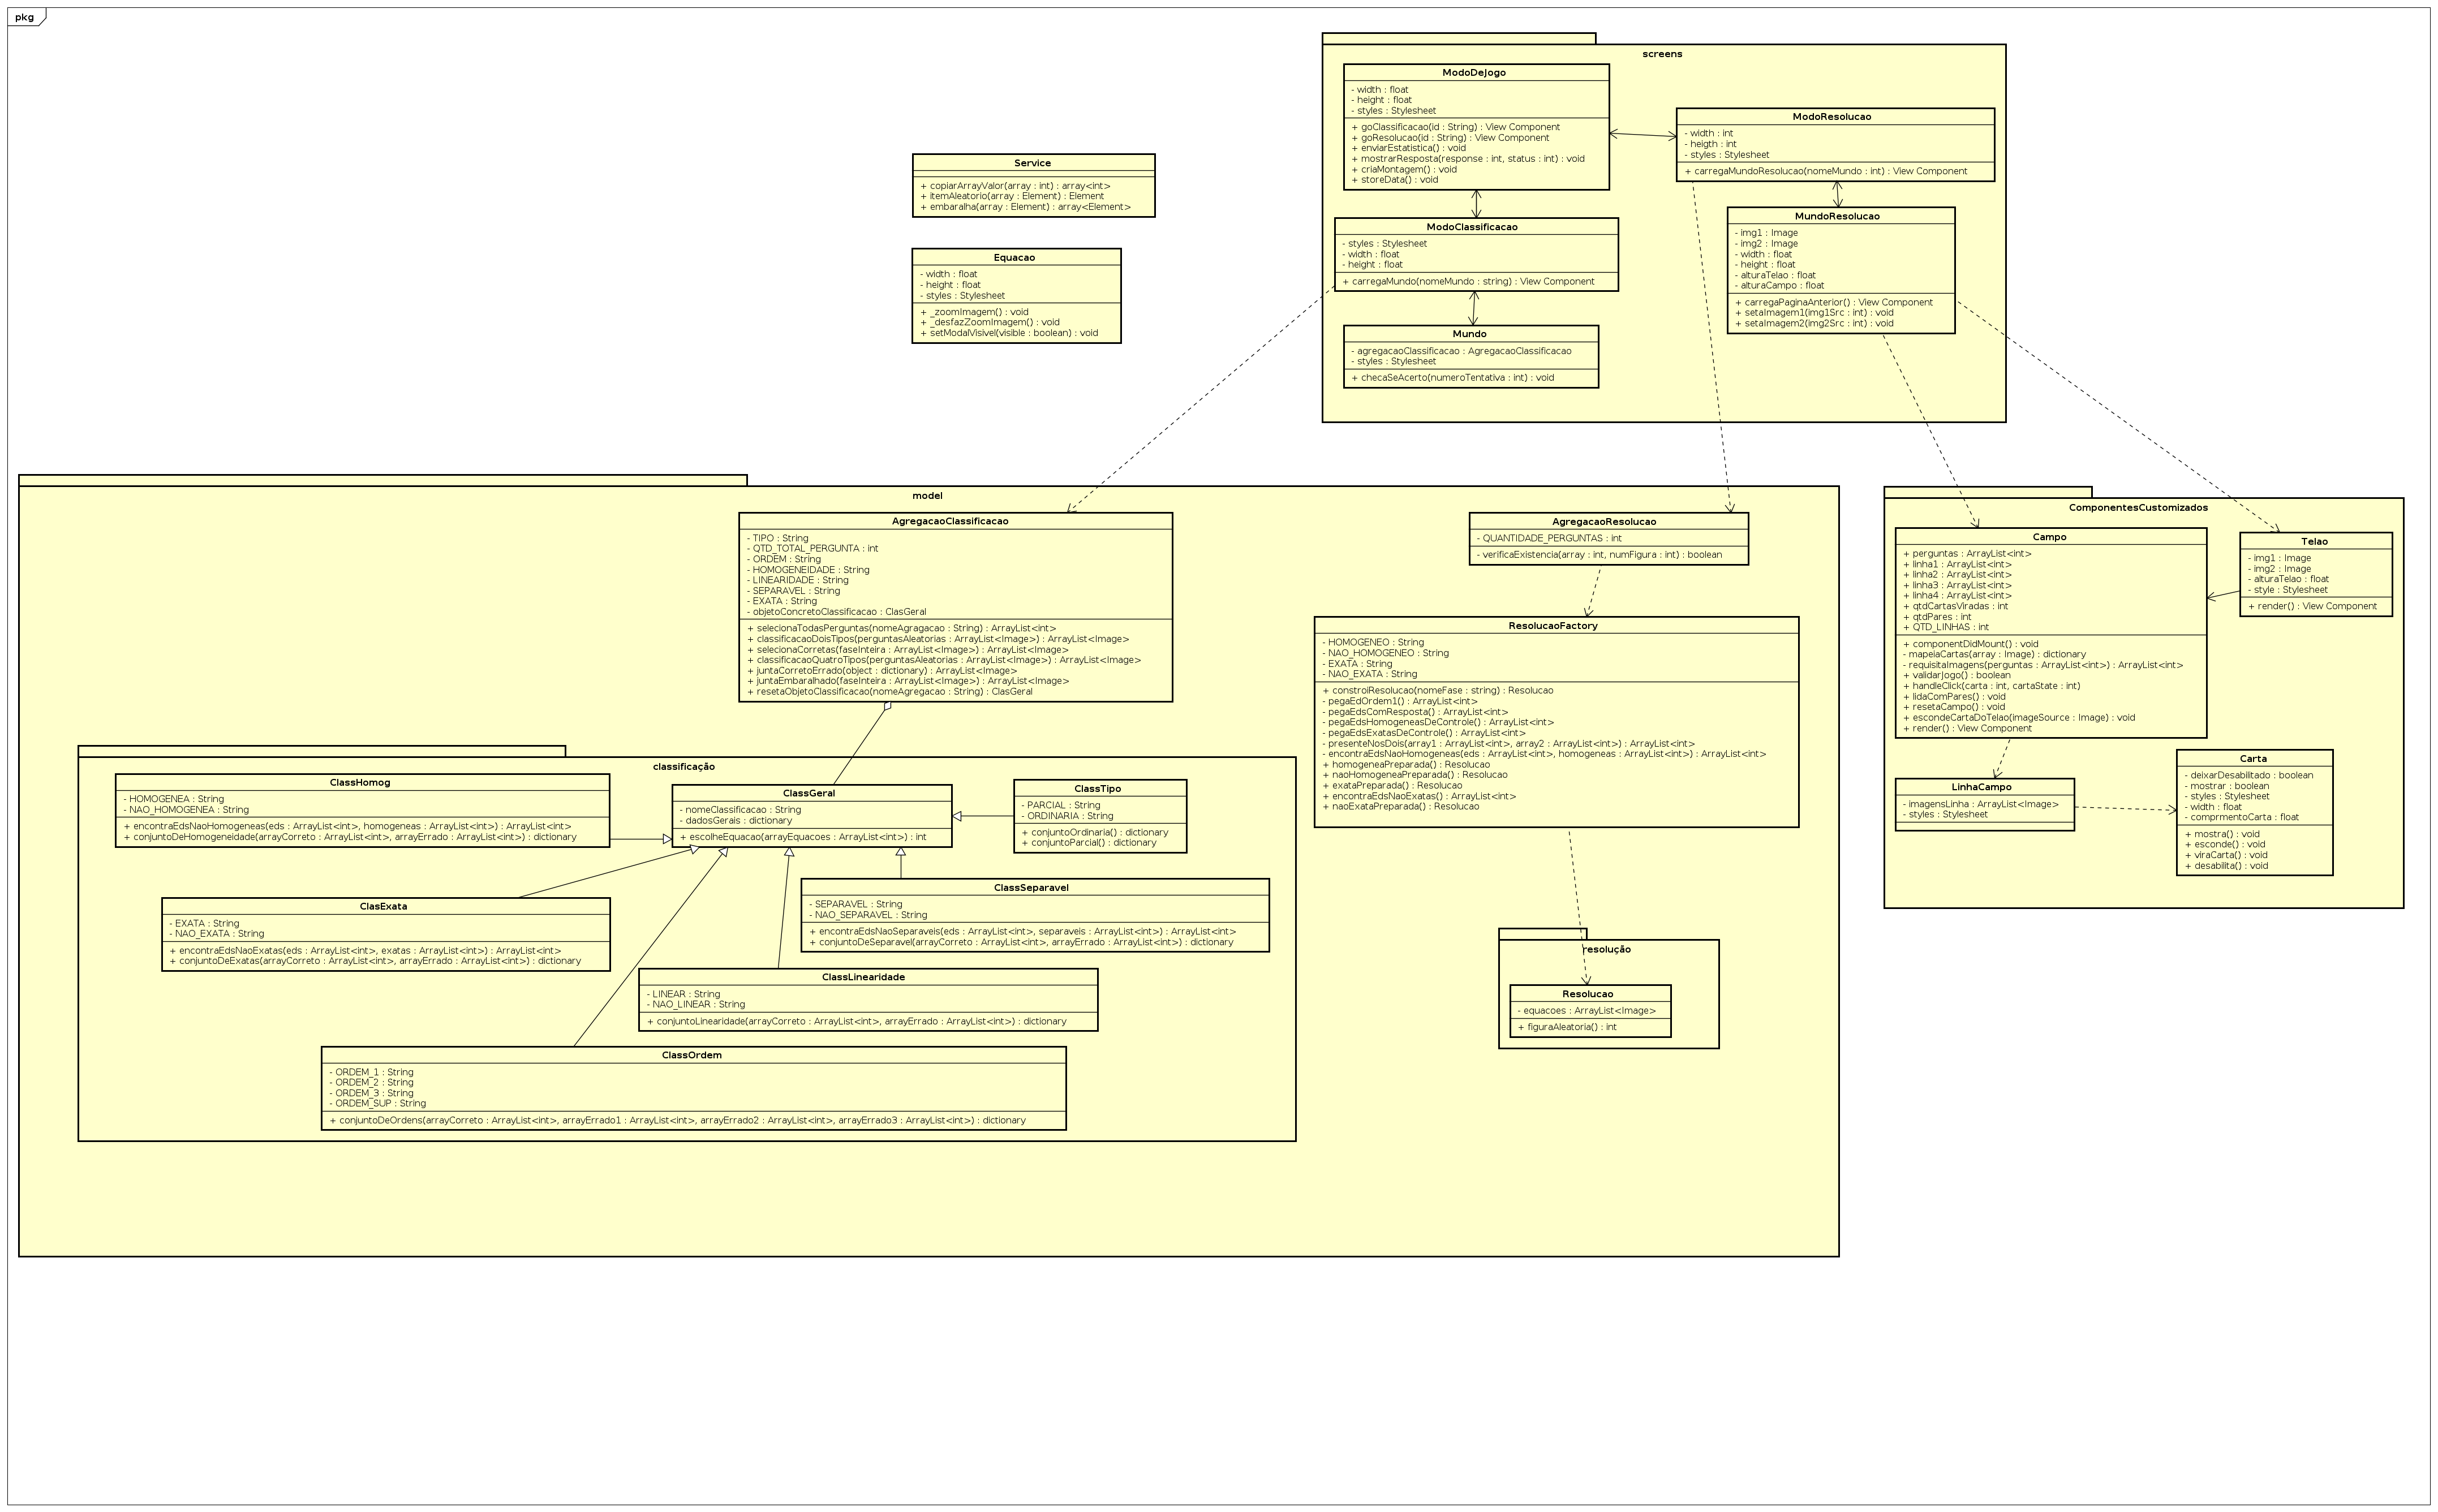
\includegraphics[width=\textwidth,height=\textheight,keepaspectratio]{figuras/DC_novo2.png}
\small{Fonte: do próprio autor}
\end{figure}

A pasta src apresenta o código fonte escrito em React (node.js).
A modelagem da aplicação é possível visualizar no diagrama de classe. Tem-se a pasta dos componentes customizados, a pasta model (que tem o modelo de perguntas e respostas e classes construtoras da agregação de perguntas e respostas para o jogo),  a pasta screens que contém as telas de jogo, sendo que algumas screens contém componentes que estão na pasta de componentes customizados. Tem o arquivo Service.js que realiza algumas tarefas auxiliares necessárias em partes misturadas do jogo, como por exemplo embaralhar um array (conjunto de dados homogêneos), realizar uma cópia de valores de um array e escolher um item aleatório.

\begin{comment}
VARIÁVEIS  

agregaçãoResolução
\label{agregaçãoResolução}

agregacaoClassificação
\label{agregacaoClassificação}

primeira\_vez
\label{primeira_vez}

mundo\_resolucao
\label{mundo_resolucao}

todasPerguntas
\label{todasPerguntas}

imgSrc
\label{imgSrc}
\end{comment}

A seguir uma explicação das funções desenvolvidas que estão na pasta SRC.

\textbf{PASTA: SRC}
\begin{itemize}
\item ARQUIVO:Service
\end{itemize}
copiarArrayValor: recebe um vetor como parâmetro e copia apenas os seus valores sem manter a referência. Para isso criar um vetor vazio, percorre o recebido e escreve seus valores no novo vetor que será retornado.

itemAleatorio: recebe um vetor como parâmetro. Em caso de não pelo menos um elemento, nulo é retornado. Caso contrário com o apoio da biblioteca Math de matemática, um número flutuante entre 0 e 1 é escolhido e multiplicado pelo comprimento do vetor. O número é arredondado para baixo e então o item nesta posição do vetor é retornado.

embaralha: recebe um vetor e aleatoriamente troca as posições dos valores

\begin{itemize}
	\item ARQUIVO:Equacao
\end{itemize}

\_zoomImagem
\label{_zoomImagem}: função ativada quando houver um longo clique em cima de algum exemplo de equação. Esta habilita o aparecimento de uma modal para mostrar equação ampliada.

\_desfazZoomImagem
\label{_desfazZoomImagem}: função ativada quando o dedo é tirado da tela após um longo clique em cima de algum exemplo de equação. Esta desabilita o aparecimento de uma modal que mostra equação ampliada.

setModalVisivel: função chamada por \hyperref[_zoomImagem]{\_zoomImagem} e \hyperref[_desfazZoomImagem]{\_desfazZoomImagem} para habilitar ou desabilitar o aparacimento da modal com equação ampliada.



\textbf{PASTA:SRC/screens}
\begin{itemize}
\item ARQUIVO:ModoDeJogo
\end{itemize}
goClassificacao: a função goClassificacao utiliza a dependência Navigation e serve para redirecionar para a tela de classificação das equações diferenciais. Recebe como parâmetro um ID que é um identificador único do tipo string referente ao nome da screen que é para redirecionar.

goResolucao: a função goResolucao utiliza a dependência Navigation importada no projeto que serve para redirecionar para a tela de resolução das equações diferenciais. Recebe como parâmetro um ID que é um identificador único do tipo string referente ao nome da screen que é para redirecionar.

enviarEstatísticas: a função enviarEstatisticas funciona de modo assíncrono e utiliza da dependência netInfo para checar seu dispositivo está conectado à internet. Caso o dispositivo não esteja, um alerta avisando ao usuário que não está conectado à Internet é acionado e retorna a página inicial da aplicação, caso haja conexão com a internet é checado se a matrícula digitada pelo usuário não é nula e ao remover os caracteres de barra de espaço verifica-se que não está vazio e que contém 8 dígitos. Em caso de matrícula inserida corretamente é acionado um loader enquanto as estatísticas locais do celular são capturados e formatadas para então realizar uma requisição ao servidor do Heroku na rota ‘/estatísticas’. O conteúdo JSON é formatado para string e então enviado. Após o processamento no servidor uma resposta é retornada para o aplicativo e a função enviarEstatisticas chama a função mostraResposta que tratará de mostrar a resposta adequada a depender do status de retorno do Servidor. Em caso de alguma exceção ocorrer durante todo o processamento um alerta é mostrado ao usuário indicando que houve erro com o servidor e pedindo para retornar mais tarde. O loader é desabilitado e novamente retorna-se a tela inicial da aplicação.

mostraResposta: a função mostraResposta é acionada pela função enviarEstatisticas e também assíncrona. Recebe como parâmetro a resposta do Servidor e o código de status. Caso a resposta tenha sucesso NÃO OKAY é mostrado um alerta para o usuário informando retorno não esperado e retorna-se à tela inicial. Em caso de resposta sucesso OKAY é carregado da memória local as estatísticas atuais e um loop percorre todas as fases do modo de classificação e de resolução zerando a quantidade de vezes que o jogador terminou de jogar, para que no próximo envio seja enviado apenas as variações entre o último envio e o atual. Após as estatísticas estarem zeradas, sstas são salvas na memória do celular e um alerta de estatísticas enviadas com sucesso é apresentado ao usuário, só então retorna-se a tela inicial.

\label{criaMontagem}: a função é acionada apenas na primeira vez o que o jogador acessa o jogo para então criar o template das estatísticas de classificação e resolução e todas as suas fases e assim é salvo na memória do celular. O tipo de dado das estatísticas é um Json.

storeData: a função storeData é acionada toda vez que um jogador entra no jogo. É tentado recuperar da memória uma variável chamada \ref{primeira_vez}, caso esta variável seja nula significa que é a primeira vez do usuário no jogo, esta variável é então criada e salva na memória com valor falso para nas outras vezes não cair neste caso, chama-se a função \ref{criaMontagem} para gerar o template das estatísticas. Caso a variável \ref{primeira_vez} já exista e retorne o valor de falso, significa que não é a primeira vez do usuário no jogo e nada acontece.

\begin{itemize}
\item ARQUIVO:ModoClassificacao
\end{itemize}
carregaMundo: função assíncrona que tem como parâmetro o nome de mundo que será criado para ser repassado ao objeto agregação classificação. Este objeto serve para a função na hora de chamar a nova tela de mundo passando as propriedades: vetor de perguntas aleatórias criadas, vetor do número das imagens corretas, vetor das fases embaralhadas, o total de questões e o nome do mundo.

\begin{itemize}
\item ARQUIVO:ModoResolucao
\end{itemize}	
carregaMundoResolucao: função assíncrona que recebe como parâmetro o nome do mundo para criar objeto agregaçãoResolução e passar para próxima \textit{screen} chamada \ref{mundo_resolução} junto com a propriedade \ref{todasPerguntas} que é um vetor provido pelo objeto agregaçãoResolução

\begin{itemize}
\item ARQUIVO:Mundo
\end{itemize}	
checaSeAcerto: função assíncrona é ativada assim que alguma opção de classificação é clickada. Recebe como parâmetro o número da tentativa da rodada, que varia de 1 a 4. Caso o número da tentativa clicada seja igual ao da pergunta correta o número da perguntaAtual é incrementado e o número da quantidade de perguntasCorretas também é incrementado apenas em caso de não ser a última pergunta. Em caso de ser a última pergunta e tentativa estiver correta as estatísticas são atualizadas com o incremento de uma vitória na fase jogada do módulo de classificação. Ao vencer a fase um alerta de parabenização é mostrado e abre-se uma janela que ao ser confirmada retorna à tela de classificação. No caso de tentativa incorreta é mostrado um alerta de tente novamente e retorna-se à questão pendente. 

\begin{itemize}
\item ARQUIVO:MundoResolucao
\end{itemize}
carregaPaginaAnterior: utiliza a dependência Navigation e apenas fecha a página atual que a página anterior já está na pilha e passa então a ser a atual.


\textbf{PASTA:SRC/model}


\textbf{PASTA:SRC/ComponentesCustomizados}
\begin{itemize}
\item ARQUIVO:Campo
\end{itemize}

mapeiaCartas: recebe o array retornado da requisitaImagens o qual inicia-se com uma pergunta e sucessivamente sua solução. Um loop é feito no array para criar um dicionário com chaves as perguntas e valor as respostas. Por isso o loop é iterado apenas nas perguntas, que são as posições pares. Ao final da iteração e população do dicionário, o mesmo é retornado.
	
requisitaImagens: recebe um array com o número das figuras aleatórias sorteadas para esta partida e faz o import através da função require procurando no arquivo index das perguntas e das respostas. O retorno é um array com 20 figuras, sendo 10 perguntas e 10 soluções das perguntas. OBS: o array de retorno é ordenado com uma pergunta e a sua solução sucessivamente.

validarJogo: é chamada sempre que duas cartas estão viradas para cima. A função serve para decidir se duas cartas formam um par. A verificação ocorre comparando com o array de cartas mapeado chave e valor. O procedimento checa se a primeira carta virada é chave ou valor. Se for chave, então compara a segunda carta com o valor, se for valor, procura-se então a chave para comparar com a segunda carta para assim confirmar se a dupla forma um par gêmeo ou não. Em caso de ser um par, pela regra do jogo é decrementado uma unidade dos pares restantes, se for o último par já acontece a atualização das estatísticas de qual fase do módulo resolução foi vencido e a parabenização ao usuário com retorno para a tela de escolha de fase. Se não for o último par, a função apenas retorna informando se as cartas atuais formam um par ou não.


handleClick: é acionada quando ocorre o click em qualquer carta enviando a informação se a carta é para ser virada ou escondida (true ou false). Se for um click para mostrar a carta, então a variável quantidadeDeCartasViradas é incrementado em 1. 
	OBS: Se esta for a única carta virada então na posição reservada para a imagem 1 será renderizada a equação da carta
	OBS1: Se for a segunda carta virada, a carta será desenhada no espaço reservado para a imagem 2 e será aplicado o procedimento do jogo da memória para validar se as 2 cartas foram um par. 

Se for um click para não mostrar a carta é acionada a função para esconder a carta do telão (espaço reservado para renderização das equações), e se o valor da variável não cair em nenhum dos casos previstos um novo erro é lançado.

lidaComPares: é chamada pelo handleClick deste mesmo arquivo. Recebe como parâmetro um booleano que representa se as duas cartas viradas para cima formam um par ou não. Em caso de serem um par, as cartas tem a função de click desabilitadas, e são travadas viradas pra cima com a imagem da equação sendo mostrada. Em caso de não serem um par as duas são viradas para o lado inverso escondendo o seu conteúdo. 

resetaCampo: esta função limpa as 2 equações renderizadas no telão, altera o estado de quantidadeDeCartasViradas para 0 e limpa o vetor de 2 posições que armazena as cartas viradas no momento.

escondeCartaDoTelao: recebe como parâmetro a imgSrc da imagem a ser escondida. Para isso também é necessário decrementar a quantidade de cartas viradas em uma unidade e então checar qual das duas cartas do telão que tem a imgSrc igual ao que foi passado para esta função, para então poder setá-lo como nulo. 

\begin{itemize}
\item ARQUIVO:Telao
\end{itemize}	


\begin{itemize}
\item ARQUIVO:LinhaCampo
\end{itemize}

	encaminha a função handle para cada carta do campo assim como o conteúdo da carta também, ou seja, a sua imagem, seja uma carta de pergunta, ou de resposta.
 
\begin{itemize}
\item ARQUIVO:Carta
\end{itemize}
mostra: alterna o estado da variável mostrar e troca o valor da animação de 0 graus para 180 graus, realizando o efeito de virar a carta.

esconde: alterna o estado da variável mostrar e troca o valor da animação de 180 graus para 0 graus, realizando o efeito de virar a carta e mostrar o fundo.

viraCarta: checa o estado da variável mostrar para decidir se chama a função mostra ou esconde e chama a função handle que lida com as regras do jogo da memória.

desabilita: troca o estado da variável deixarDesabilitado, a qual é chamada apenas quanto um par de cartas gêmeas é encontrado. Desse modo impede que a carta seja rotacionada desse momento para frente, deixando-a sempre virada com a parte do conteúdo para cima, porém desabilitada para cliques.


\section[Servidor aprEnDO]{Servidor aprEnDO}
O servidor aprendo hospedado no heroku serve para receber estatísticas dos aplicativos enviados pelos alunos. Os alunos para enviar a estatística precisam informar o número da matrícula. As informações são enviadas em formato JSON e armazenadas no banco de dados integrado com o servidor.

O jogo aprEnDO além do aplicativo de celular tem um servidor para contabilizar dados do jogo.
O servidor está hospedado no heroku utilizando uma contra free que esteve disponível durante a fase de teste dos alunos, apesar de gratuito comparado com a necessidade que era necessário deu para suprir todas as expectativas. Junto com a aplicação foi adicionado um plugin de banco de dados mongodb. Este banco armazenou em um documento os metadados do jogo. O mongodb é um add-on no mLab que permite integração com o heroku, ele permite uma conta temporária com uma quantidade limitada de capacidade de dados, mas para o necessário que são apenas arquivo json. O único problema é que  o mLab não recomenda utilizar a conta free para a produção por não produzir replicação, porém o banco estava sendo acompanhado muitas vezes por dia para coletar os dados recebidos dos alunos. 
O servidor foi escrito em node.js. O script index.js do servidor cria uma rota /estatísticas que é a utilizada pelos aplicativos para enviar a requisição POST. 

O servidor está hospedado no github do heroku, pela interface da linha de comando (CLI) pode ser clonado o projeto com o comando 'heroku git:clone -a servidor-aprendo'.
Para desenvolvimento foi utilizado uma única branch, que foi o necessário. Mais branches seriam criadas, caso fosse necessário. Tendo em vista que o servidor deveria estar pronto até o dia 10 de maio, que era o início da data de aplicação do jogo com os alunos, até esta data o servidor estava sendo desenvolvido e testado, o único problema crucial que poderia ocorrer seria não realizar os commits dos códigos adicionados e removidos. Assim que o servidor estivesse pronto, a expectativa era não precisar alterar mais código nele, apenas se o servidor quebrasse por algum caso inesperado, aí sim o servidor teria de entrar no ar novamente e novas branches de correção seriam criadas para não impedir o funcionamento parcial do servidor. Porém como os logs do servidor estavam sendo acompanhados muitas vezes por dia durante o período de aplicação e o servidor não caiu nenhuma vez, não foi necessário criar branches adicionais para a correção de erros. 

Ao receber os dados json enviados do aplicativo do celular para o servidor, o mesmo concatena todos os dados que chegam em uma variável apenas. Ao terminar a leitura dos dados de chegada eles são formatados é escrito uma resposta de sucesso verdadeiro, a função ‘lê histórico’ é chamada e a resposta é encerrada.

A função ‘lê histórico’ recupera o documento existente no banco de dados heroku\_41w8651l hospedado no mLab, da coleção chamada histórico. A função analisa checa se a matrícula recebida pela requisição já havia alguma vez enviado estatísticas ou se é uma matrícula nova. Em caso de matrícula nova, uma nova linha é adicionada com chave primária a matrícula do aluno e salva no banco. Em caso de matrícula existente é iterado sobre classificação e resolução e todas suas fases e incrementado a quantidade de vitórias a mais que foi concluído das fases no jogo e em seguida o arquivo é atualizado no banco do mLab.

\section[Acesso ao código]{Acesso ao código}
O código do servidor está hospedado no github do heroku, disponível em \url{https://dashboard.heroku.com/apps/servidor-aprendo}.

Todo o código está hospedado no github. O banco de equações e a aplicação para android estão disponíveis no seguinte link \url{https://github.com/LeonardoRk/TCC-2}.


O APP publicado no google play pode ser encontrado através do link: \url{https://play.google.com/store/apps/details?id=projeto.aprEnDO&rdid=projeto.aprEnDO}

E a biblioteca do Wolfran Alpha em javascript pode ser baixada no link: \url{https://products.wolframalpha.com/api/libraries.html}. Porém a biblioteca já está inclusa no github dentro da pasta banco.

\section[Empacotamento]{Empacotamento}
O jogo é empacotado para criar um arquivo .apk, e este que é instalado nos celulares. Para submeter o jogo ao Google Play para os jogadores poderem baixá-lo é necessário criar o .apk. O mesmo só é criado sempre que tem alguma nova atualização no jogo, seja no banco de equações ou manutenção corretiva ou evolutiva do jogo.

O empacotamento do jogo ocorre dentro da pasta do projeto react native. É utilizado o comando 'npm run android'.



\begin{comment}
////
A respeito do jogo, como colher dados? Os dados são colhidos quando o jogador está utilizando o jogo. Porém o dados são mantidos apenas no dispositivo. A pessoa pode enviar a estatística quando desejar, o professor solicitará o envio constante dos dados dos alunos.

Como enviar estatísticas? Haverá um botão responsável de enviar estatísticas, que podem ser enviadas para o servidor através do jogo em apenas um clique e uma confirmação do jogador. Assim que enviadas, as estatísticas armazenadas no celular se apagam para que no próximo envio não hajam informações repetidas.

Os dados colhidos e enviados são separados fase e módulos.

Por pergunta:\\
	- Qual é a pergunta alvo\\
	- Número das 4 EDs\\
	- Quantas tentativas foram necessárias para acertar a pergunta. **para saber se clicam aleatório ou escolhem antes de clicar **\\
	- Tempo gasto em cada pergunta  **para saber se a tela não ficou parada e o celular sem atenção**\\

	Algumas observações são: o clique pode demorar para acontecer ou acontecer muito rápido e as consequências podem ser acertar de primeira ou não acertar de primeira.\\
	Algumas inferências são: 
	cliques muito rápidos e não acertar de primeira == PODE significar chute aleatório\\
	cliques muito rápidos e acertar de primeira == pode ser um robô? alunos muito bem preparados?\\
	cliques devagar e não acertar de primeira == tá muito difícil? O celular está parado? \\
	cliques devagar e acertar de primeira == estava pensando? Estava resolvendo? O celular estava parado?\\

Por fase:\\
	- Quanto tempo durou cada fase (de 20 perguntas)\\

Dentro de cada módulo:\\
	- Quantas vezes clickou para jogar em uma fase(linear,exata,etc..) de classificação e saiu? (após 3 \\segundos)
	- Quantas vezes clickou para jogar em uma fase(homog, exata, etc) de resolução e saiu? (após 3 \\segundos)
	- Tempo total no módulo de classificação\\
	- Tempo total no módulo de resolução\\
	- Quantas vezes entrou e saiu de cada módulo (considerar que saiu é após 3 segundos).\\


Quantas vezes cada módulo foi clickado para jogar, e quantas ficaram sendo jogados mesmo.

Será avaliado dos mapas conceituais se houve evolução significativa entre os mapas conceituais dos alunos participantes em relação aos não participantes do jogo.
As estatísticas do jogo será para avaliar o desempenho dos alunos e qual a aceitação do jogo pelos participantes, para saber se é uma estratégia que pode ser levada adiante ou não.
\end{comment}
